% Options for packages loaded elsewhere
\PassOptionsToPackage{unicode=true}{hyperref}
\PassOptionsToPackage{hyphens}{url}
\PassOptionsToPackage{dvipsnames,svgnames*,x11names*}{xcolor}
%
\documentclass[
]{article}
\usepackage{lmodern}
\usepackage{amssymb,amsmath}
\usepackage{ifxetex,ifluatex}
\ifnum 0\ifxetex 1\fi\ifluatex 1\fi=0 % if pdftex
  \usepackage[T1]{fontenc}
  \usepackage[utf8]{inputenc}
  \usepackage{textcomp} % provides euro and other symbols
\else % if luatex or xelatex
  \usepackage{unicode-math}
  \defaultfontfeatures{Scale=MatchLowercase}
  \defaultfontfeatures[\rmfamily]{Ligatures=TeX,Scale=1}
\fi
% Use upquote if available, for straight quotes in verbatim environments
\IfFileExists{upquote.sty}{\usepackage{upquote}}{}
\IfFileExists{microtype.sty}{% use microtype if available
  \usepackage[]{microtype}
  \UseMicrotypeSet[protrusion]{basicmath} % disable protrusion for tt fonts
}{}
\makeatletter
\@ifundefined{KOMAClassName}{% if non-KOMA class
  \IfFileExists{parskip.sty}{%
    \usepackage{parskip}
  }{% else
    \setlength{\parindent}{0pt}
    \setlength{\parskip}{6pt plus 2pt minus 1pt}}
}{% if KOMA class
  \KOMAoptions{parskip=half}}
\makeatother
\usepackage{xcolor}
\IfFileExists{xurl.sty}{\usepackage{xurl}}{} % add URL line breaks if available
\IfFileExists{bookmark.sty}{\usepackage{bookmark}}{\usepackage{hyperref}}
\hypersetup{
  pdftitle={Movie Recommendation System - Capstone Project},
  pdfauthor={Mitja Prah - HarvardX Data Science Professional Program},
  colorlinks=true,
  linkcolor=Maroon,
  filecolor=Maroon,
  citecolor=Blue,
  urlcolor=blue,
}
\urlstyle{same} % disable monospaced font for URLs
\usepackage[margin=1in]{geometry}
\usepackage{color}
\usepackage{fancyvrb}
\newcommand{\VerbBar}{|}
\newcommand{\VERB}{\Verb[commandchars=\\\{\}]}
\DefineVerbatimEnvironment{Highlighting}{Verbatim}{commandchars=\\\{\}}
% Add ',fontsize=\small' for more characters per line
\newenvironment{Shaded}{}{}
\newcommand{\AlertTok}[1]{\textcolor[rgb]{1.00,0.00,0.00}{\textbf{#1}}}
\newcommand{\AnnotationTok}[1]{\textcolor[rgb]{0.38,0.63,0.69}{\textbf{\textit{#1}}}}
\newcommand{\AttributeTok}[1]{\textcolor[rgb]{0.49,0.56,0.16}{#1}}
\newcommand{\BaseNTok}[1]{\textcolor[rgb]{0.25,0.63,0.44}{#1}}
\newcommand{\BuiltInTok}[1]{#1}
\newcommand{\CharTok}[1]{\textcolor[rgb]{0.25,0.44,0.63}{#1}}
\newcommand{\CommentTok}[1]{\textcolor[rgb]{0.38,0.63,0.69}{\textit{#1}}}
\newcommand{\CommentVarTok}[1]{\textcolor[rgb]{0.38,0.63,0.69}{\textbf{\textit{#1}}}}
\newcommand{\ConstantTok}[1]{\textcolor[rgb]{0.53,0.00,0.00}{#1}}
\newcommand{\ControlFlowTok}[1]{\textcolor[rgb]{0.00,0.44,0.13}{\textbf{#1}}}
\newcommand{\DataTypeTok}[1]{\textcolor[rgb]{0.56,0.13,0.00}{#1}}
\newcommand{\DecValTok}[1]{\textcolor[rgb]{0.25,0.63,0.44}{#1}}
\newcommand{\DocumentationTok}[1]{\textcolor[rgb]{0.73,0.13,0.13}{\textit{#1}}}
\newcommand{\ErrorTok}[1]{\textcolor[rgb]{1.00,0.00,0.00}{\textbf{#1}}}
\newcommand{\ExtensionTok}[1]{#1}
\newcommand{\FloatTok}[1]{\textcolor[rgb]{0.25,0.63,0.44}{#1}}
\newcommand{\FunctionTok}[1]{\textcolor[rgb]{0.02,0.16,0.49}{#1}}
\newcommand{\ImportTok}[1]{#1}
\newcommand{\InformationTok}[1]{\textcolor[rgb]{0.38,0.63,0.69}{\textbf{\textit{#1}}}}
\newcommand{\KeywordTok}[1]{\textcolor[rgb]{0.00,0.44,0.13}{\textbf{#1}}}
\newcommand{\NormalTok}[1]{#1}
\newcommand{\OperatorTok}[1]{\textcolor[rgb]{0.40,0.40,0.40}{#1}}
\newcommand{\OtherTok}[1]{\textcolor[rgb]{0.00,0.44,0.13}{#1}}
\newcommand{\PreprocessorTok}[1]{\textcolor[rgb]{0.74,0.48,0.00}{#1}}
\newcommand{\RegionMarkerTok}[1]{#1}
\newcommand{\SpecialCharTok}[1]{\textcolor[rgb]{0.25,0.44,0.63}{#1}}
\newcommand{\SpecialStringTok}[1]{\textcolor[rgb]{0.73,0.40,0.53}{#1}}
\newcommand{\StringTok}[1]{\textcolor[rgb]{0.25,0.44,0.63}{#1}}
\newcommand{\VariableTok}[1]{\textcolor[rgb]{0.10,0.09,0.49}{#1}}
\newcommand{\VerbatimStringTok}[1]{\textcolor[rgb]{0.25,0.44,0.63}{#1}}
\newcommand{\WarningTok}[1]{\textcolor[rgb]{0.38,0.63,0.69}{\textbf{\textit{#1}}}}
\usepackage{longtable,booktabs}
% Allow footnotes in longtable head/foot
\IfFileExists{footnotehyper.sty}{\usepackage{footnotehyper}}{\usepackage{footnote}}
\makesavenoteenv{longtable}
\usepackage{graphicx,grffile}
\makeatletter
\def\maxwidth{\ifdim\Gin@nat@width>\linewidth\linewidth\else\Gin@nat@width\fi}
\def\maxheight{\ifdim\Gin@nat@height>\textheight\textheight\else\Gin@nat@height\fi}
\makeatother
% Scale images if necessary, so that they will not overflow the page
% margins by default, and it is still possible to overwrite the defaults
% using explicit options in \includegraphics[width, height, ...]{}
\setkeys{Gin}{width=\maxwidth,height=\maxheight,keepaspectratio}
\setlength{\emergencystretch}{3em} % prevent overfull lines
\providecommand{\tightlist}{%
  \setlength{\itemsep}{0pt}\setlength{\parskip}{0pt}}
\setcounter{secnumdepth}{5}
% Redefines (sub)paragraphs to behave more like sections
\ifx\paragraph\undefined\else
  \let\oldparagraph\paragraph
  \renewcommand{\paragraph}[1]{\oldparagraph{#1}\mbox{}}
\fi
\ifx\subparagraph\undefined\else
  \let\oldsubparagraph\subparagraph
  \renewcommand{\subparagraph}[1]{\oldsubparagraph{#1}\mbox{}}
\fi

% Set default figure placement to htbp
\makeatletter
\def\fps@figure{htbp}
\makeatother

\usepackage{booktabs}
\usepackage{longtable}
\usepackage{array}
\usepackage{multirow}
\usepackage{wrapfig}
\usepackage{float}
\usepackage{colortbl}
\usepackage{pdflscape}
\usepackage{tabu}
\usepackage{threeparttable}
\usepackage{threeparttablex}
\usepackage[normalem]{ulem}
\usepackage{makecell}
\usepackage{xcolor}

\title{Movie Recommendation System - Capstone Project}
\author{Mitja Prah - HarvardX Data Science Professional Program}
\date{26/11/2020}

\begin{document}
\maketitle

{
\hypersetup{linkcolor=}
\setcounter{tocdepth}{3}
\tableofcontents
}
\newpage

\hypertarget{overview}{%
\section{Overview}\label{overview}}

Recommendation systems use ratings that users have given items to make
specific recommendations to users. Companies like Amazon that sell many
products to many customers and permit these customers to rate their
products are able to collect massive datasets that can be used to
predict what rating a given user will give a specific item. Items for
which a high rating is predicted for specific users are then recommended
to that user.

Netflix used recommendation systems to predict how many stars a user
would give a specific movie. On October 2006, Netflix offered a
challenge to the data science community: \emph{``Improve our
recommendation algorithm by 10\% and win \$1 million.''} For more
information about the ``Netflix Challenge,'' you can check out these
sites:

\begin{itemize}
\tightlist
\item
  \url{https://bits.blogs.nytimes.com/2009/09/21/netflix-awards-1-million-prize-and-starts-a-new-contest/}~\\
\item
  \url{http://blog.echen.me/2011/10/24/winning-the-netflix-prize-a-summary/}~\\
\item
  \url{https://www.netflixprize.com/assets/GrandPrize2009_BPC_BellKor.pdf}
\end{itemize}

For our project, we will try to take a similar challenge. We will be
creating a movie recommendation system using the MovieLens dataset,
which describes millions of movie ratings and tagging activity from
MovieLens, a movie recommendation service.

Recommendation systems are complicated machine learning challenges
because each outcome has a different set of predictors. For example,
different users rate a different number of movies and rate different
movies.

To compare different models or to see how well we're doing compared to a
baseline, we can use Root Mean Squared Error (RMSE) as our \emph{loss
function}. We define \(y_{u,i}\) as the rating for movie \(i\) by user
\(u\) and denote our prediction with \(\hat{y}_{u,i}\). The RMSE is then
defined as:

\[
\mbox{RMSE} = \sqrt{\frac{1}{N} \sum_{u,i}^{} \left( \hat{y}_{u,i} - y_{u,i} \right)^2 }
\] with \(N\) being the number of user/movie combinations and the sum
occurring over all these combinations.

We can interpret RMSE similar to standard deviation - it is the typical
error we make when predicting a movie rating. If this number is larger
than 1, it means our typical error is larger than one star, which is not
good.

\hypertarget{project-objective}{%
\subsection{Project Objective}\label{project-objective}}

Different machine learning algorithms will be evaluated in our project.
Our target is to create a model, that will be able to predict the movie
rating based on the user and movie characteristics. Finally, the most
accurate of the models will be selected based on the lowest RMSE, that
should ideally be \textbf{\textless0.86490}. If this is not reachable,
we will select the model that gets the closest to this goal.

The selected algorithm will finally be tested on the validation set. The
aim of this final evaluation will be to reach the RMSE of
\textbf{\textless0.86490}, as our primary project objective.

The following function will be used in this project, and will compute
the RMSE for vectors of ratings and their corresponding predictors:

\begin{Shaded}
\begin{Highlighting}[]
\CommentTok{#RMSE function}
\NormalTok{RMSE <-}\StringTok{ }\ControlFlowTok{function}\NormalTok{(true_ratings, predicted_ratings)\{}
  \KeywordTok{sqrt}\NormalTok{(}\KeywordTok{mean}\NormalTok{((true_ratings }\OperatorTok{-}\StringTok{ }\NormalTok{predicted_ratings)}\OperatorTok{^}\DecValTok{2}\NormalTok{))}
\NormalTok{\}}
\end{Highlighting}
\end{Shaded}

\hypertarget{dataset-and-data-collection}{%
\subsection{Dataset and Data
Collection}\label{dataset-and-data-collection}}

The full latest MovieLens dataset is available here:
\url{https://grouplens.org/datasets/movielens/latest/}.

To simplify this data science project, I will use the smaller 10M
version of the MovieLens dataset, available on:
\url{https://grouplens.org/datasets/movielens/10m/}. It contains 100,836
ratings and 3683 tag applications across 9742 movies. These data were
created by 610 users between March 29, 1996 and September 24, 2018. This
dataset was generated on September 26, 2018. The dataset used for this
project is the 10M version of the MovieLens dataset, freely available
online:

\begin{itemize}
\tightlist
\item
  \url{https://grouplens.org/datasets/movielens/10m/}~\\
\item
  \url{http://files.grouplens.org/datasets/movielens/ml-10m.zip}
\end{itemize}

MovieLens users were selected at random for inclusion. All selected
users had rated at least 20 movies. No demographic information is
included. Each user is represented by an id, and no other information is
provided. This is a development dataset. As such, it may change over
time and is not an appropriate dataset for shared research results. This
and other GroupLens data sets are publicly available for download at
{[}link{]} \url{http://grouplens.org/datasets/}. For more information
about the original dataset, please reference the following paper:
\emph{F. Maxwell Harper and Joseph A. Konstan. 2015. The MovieLens
Datasets: History and Context. ACM Transactions on Interactive
Intelligent Systems (TiiS) 5, 4: 19:1--19:19.
\url{https://doi.org/10.1145/2827872}.}

\hypertarget{data-pre-processing}{%
\subsubsection{Data Pre-Processing}\label{data-pre-processing}}

The chosen primary dataset was downloaded from the above stated web
site.

The code for the initial data processing was provided in the course
HarvardX PH125.9x Data Science: Capstone. The primary dataset was split
into edx set and validation set (the final hold-out test set) in 90\% vs
10\% ratio, respectively.

The full provided code is included in the section \emph{Appendices},
\emph{Code Previously Provided by edX}, in this report.

The edx dataset is split further into edx\_train and edx\_test set, in
the ratio of 90\% vs 10\%, respectively.

All machine learning algorithms will be trained and tested on both edx
subsets. The validation set (the final hold-out test set) will ONLY be
used to test the final, best algorithm.

\newpage

\hypertarget{methods}{%
\section{Methods}\label{methods}}

\hypertarget{initial-data-exploration}{%
\subsection{Initial Data Exploration}\label{initial-data-exploration}}

\textbf{edx dataset} includes 9.000.055 observations of 6
variables/features. 10.677 different movies are rated by 69.878
different users. There are no missing values.

The 6 features are:

\begin{itemize}
\tightlist
\item
  \textbf{userId} \texttt{\textless{}integer\textgreater{}} that
  contains the unique identification number for each user.
\item
  \textbf{movieId} \texttt{\textless{}numeric\textgreater{}} that
  contains the unique identification number for each movie.
\item
  \textbf{rating} \texttt{\textless{}numeric\textgreater{}} that
  contains the rating of one movie by one user. Ratings are made on a
  5-star scale with half-star increments.
\item
  \textbf{timestamp} \texttt{\textless{}integer\textgreater{}} that
  contains the timestamp for one specific rating provided by one user.
\item
  \textbf{title} \texttt{\textless{}character\textgreater{}} that
  contains the title of each movie including the year of the release.
\item
  \textbf{genres} \texttt{\textless{}character\textgreater{}} that
  contains a list of all genres of an individual movie.
\end{itemize}

\textbf{Descriptive statistics of the edx dataset}

\begin{table}[H]
\centering\begingroup\fontsize{10}{12}\selectfont

\begin{tabular}{r|r|r|r|r|r}
\hline
N\_users & N\_movies & Mean\_rating & Median\_rating & Min\_rating & Max\_rating\\
\hline
69878 & 10677 & 3.512465 & 4 & 0.5 & 5\\
\hline
\end{tabular}
\endgroup{}
\end{table}

\textbf{The first 6 rows of the edx dataset}

\begin{table}[H]
\centering\begingroup\fontsize{10}{12}\selectfont

\resizebox{\linewidth}{!}{
\begin{tabular}{r|r|r|r|l|l}
\hline
userId & movieId & rating & timestamp & title & genres\\
\hline
1 & 122 & 5 & 838985046 & Boomerang (1992) & Comedy|Romance\\
\hline
1 & 185 & 5 & 838983525 & Net, The (1995) & Action|Crime|Thriller\\
\hline
1 & 292 & 5 & 838983421 & Outbreak (1995) & Action|Drama|Sci-Fi|Thriller\\
\hline
1 & 316 & 5 & 838983392 & Stargate (1994) & Action|Adventure|Sci-Fi\\
\hline
1 & 329 & 5 & 838983392 & Star Trek: Generations (1994) & Action|Adventure|Drama|Sci-Fi\\
\hline
1 & 355 & 5 & 838984474 & Flintstones, The (1994) & Children|Comedy|Fantasy\\
\hline
\end{tabular}}
\endgroup{}
\end{table}

\textbf{edx\_train dataset} includes 8.100.065 observations of the same
6 variables/features. 10.677 different movies were rated by 69.878
different users. There are no missing values.

\textbf{edx\_test dataset} includes 899.990 observations of the same 6
variables/features. 9.701 different movies were rated by 68.159
different users. There are no missing values.

\textbf{Validation dataset} includes 999.999 observations of the same 6
variables/features. 9.809 different movies were rated by 68.534
different users. There are no missing values.

\textbf{The first 6 rows of the validation dataset}

\begin{table}[H]
\centering\begingroup\fontsize{10}{12}\selectfont

\resizebox{\linewidth}{!}{
\begin{tabular}{r|r|r|r|l|l}
\hline
userId & movieId & rating & timestamp & title & genres\\
\hline
1 & 231 & 5 & 838983392 & Dumb \& Dumber (1994) & Comedy\\
\hline
1 & 480 & 5 & 838983653 & Jurassic Park (1993) & Action|Adventure|Sci-Fi|Thriller\\
\hline
1 & 586 & 5 & 838984068 & Home Alone (1990) & Children|Comedy\\
\hline
2 & 151 & 3 & 868246450 & Rob Roy (1995) & Action|Drama|Romance|War\\
\hline
2 & 858 & 2 & 868245645 & Godfather, The (1972) & Crime|Drama\\
\hline
2 & 1544 & 3 & 868245920 & Lost World: Jurassic Park, The (Jurassic Park 2) (1997) & Action|Adventure|Horror|Sci-Fi|Thriller\\
\hline
\end{tabular}}
\endgroup{}
\end{table}

\textbf{Descriptive statistics of the validation dataset}

\begin{table}[H]
\centering\begingroup\fontsize{10}{12}\selectfont

\begin{tabular}{r|r|r|r|r|r}
\hline
N\_users & N\_movies & Mean\_rating & Median\_rating & Min\_rating & Max\_rating\\
\hline
68534 & 9809 & 3.512033 & 4 & 0.5 & 5\\
\hline
\end{tabular}
\endgroup{}
\end{table}

\hypertarget{additional-data-processing}{%
\subsection{Additional Data
Processing}\label{additional-data-processing}}

Initial Data Exploration shows that edx and validation datasets are in
the \emph{tidy format}, suitable for further analyses. However, the
\textbf{timestamp} features are not in a human-readable format, and the
\textbf{title} features contain the information about the year, when the
movie was released. Therefore, to alleviate further data exploration and
analyses, the following additional data processing steps are performed
for all datasets:

\begin{enumerate}
\def\labelenumi{\arabic{enumi}.}
\item
  \textbf{timestamp} is converted to a human readable date format
\item
  The month and year of the movie rating, derived from the initial
  timestamp variable, are extracted from the converted timestamp
  variable
\item
  The year of the movie release is extracted from the title variable
\end{enumerate}

The \textbf{genre} features are composed of several character values,
separated by the logical \emph{or} operator (\textbar). For further
exploration of individual genres, all genres of each movie need to be
extracted at the separator values (\textbar). However, this process
requires a high computer memory consumption, and is not performed on the
edx dataset within the scope of this project for this reason.
Nevertheless, to get a rough insight on genre distributions, we will be
performing genre analyses with edx\_test dataset, which will be feasible
despite our hardware limitations. The dataset with separated individual
genres, used for genre analyses will be named
\textbf{edx\_test\_split\_genres}.

After the additional data processing and removing unnecessary columns,
the datasets have 8 variables.

\textbf{Final processed edx dataset - first 6 rows}

\begin{table}[H]
\centering\begingroup\fontsize{10}{12}\selectfont

\resizebox{\linewidth}{!}{
\begin{tabular}{r|r|r|l|l|r|r|r}
\hline
userId & movieId & rating & title & genres & year\_release & Rating\_Year & Rating\_Month\\
\hline
1 & 122 & 5 & Boomerang (1992) & Comedy|Romance & 1992 & 1996 & 8\\
\hline
1 & 185 & 5 & Net, The (1995) & Action|Crime|Thriller & 1995 & 1996 & 8\\
\hline
1 & 292 & 5 & Outbreak (1995) & Action|Drama|Sci-Fi|Thriller & 1995 & 1996 & 8\\
\hline
1 & 316 & 5 & Stargate (1994) & Action|Adventure|Sci-Fi & 1994 & 1996 & 8\\
\hline
1 & 329 & 5 & Star Trek: Generations (1994) & Action|Adventure|Drama|Sci-Fi & 1994 & 1996 & 8\\
\hline
1 & 355 & 5 & Flintstones, The (1994) & Children|Comedy|Fantasy & 1994 & 1996 & 8\\
\hline
\end{tabular}}
\endgroup{}
\end{table}

\textbf{edx\_test\_split\_genres dataset that will serve for genre
analyses - the first 6 rows}

\begin{table}[H]
\centering\begingroup\fontsize{10}{12}\selectfont

\resizebox{\linewidth}{!}{
\begin{tabular}{r|r|r|l|l|r|r|r}
\hline
userId & movieId & rating & title & genre & year\_release & Rating\_Year & Rating\_Month\\
\hline
1 & 185 & 5 & Net, The (1995) & Action & 1995 & 1996 & 8\\
\hline
1 & 185 & 5 & Net, The (1995) & Crime & 1995 & 1996 & 8\\
\hline
1 & 185 & 5 & Net, The (1995) & Thriller & 1995 & 1996 & 8\\
\hline
2 & 260 & 5 & Star Wars: Episode IV - A New Hope (a.k.a. Star Wars) (1977) & Action & 1977 & 1997 & 7\\
\hline
2 & 260 & 5 & Star Wars: Episode IV - A New Hope (a.k.a. Star Wars) (1977) & Adventure & 1977 & 1997 & 7\\
\hline
2 & 260 & 5 & Star Wars: Episode IV - A New Hope (a.k.a. Star Wars) (1977) & Sci-Fi & 1977 & 1997 & 7\\
\hline
\end{tabular}}
\endgroup{}
\end{table}

\hypertarget{further-data-exploration---data-visualisation}{%
\subsection{Further Data Exploration - Data
Visualisation}\label{further-data-exploration---data-visualisation}}

We will visualize data to get a better idea on how the number and
distribution of movie ratings vary over time and between different
movies, genres, and users. A high variability is expected due to
different popularity of movies (\emph{movie bias}) and movie genres
(\emph{genre bias}), influence of the time of movie release (\emph{time
bias}), and various personal preferences of users (\emph{user bias}).
The least rated movies and genres, and the least active users should be
given lower importance in prediction models. We will also determine the
most popular movies according to the number of ratings and according to
the mean star rating.

\newpage

\hypertarget{rating-distributions}{%
\subsubsection{Rating distributions}\label{rating-distributions}}

\textbf{Overview of Rating Distribution}

\begin{center}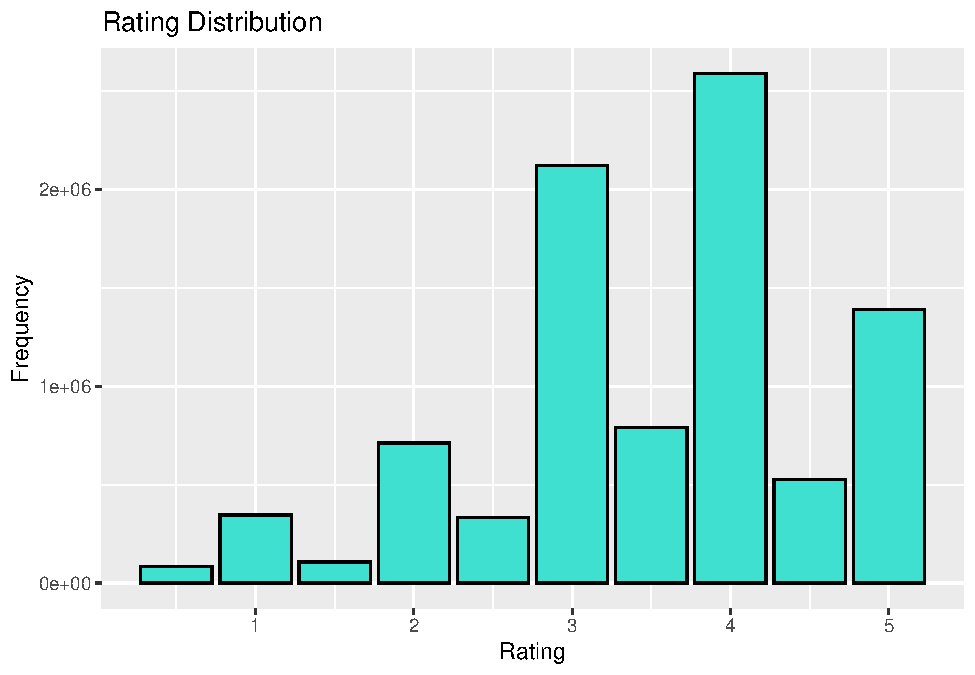
\includegraphics{MovieLens-Report_MitjaPrah_files/figure-latex/unnamed-chunk-22-1} \end{center}

The plot above shows the left-skewed distribution of the \emph{rating}
variable, revealing that there are more positive ratings (above 3 stars)
than negative ratings (below 3 stars). This could imply that users are
more inclined to rate movies that they like. We can also see that
full-star ratings are much more prevalent than half-star ratings.

\newpage

\textbf{Distribution of Number of Ratings per Year}

\begin{center}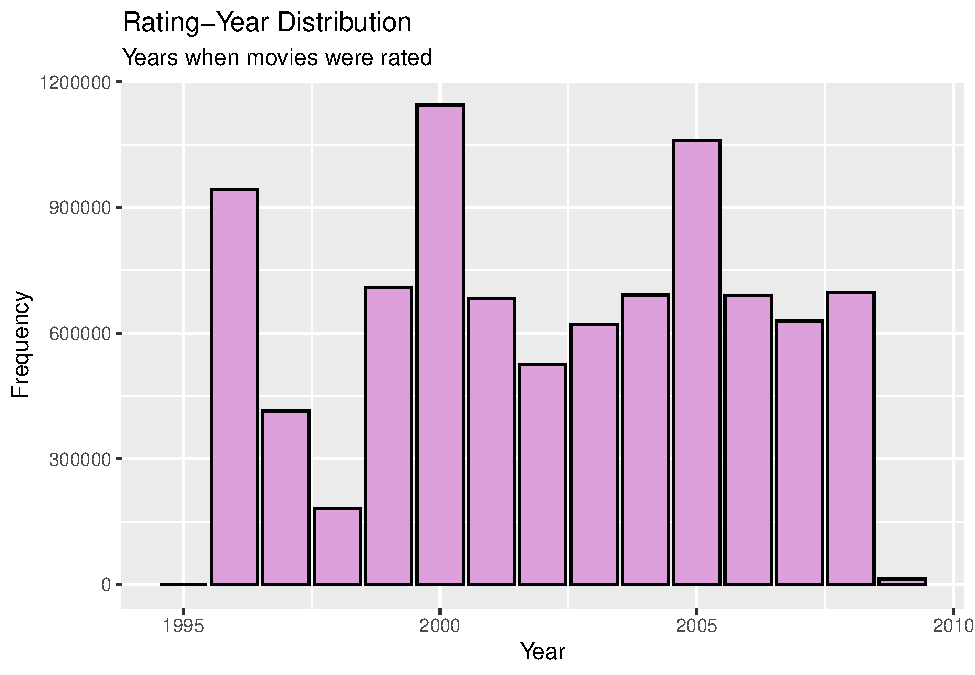
\includegraphics{MovieLens-Report_MitjaPrah_files/figure-latex/unnamed-chunk-23-1} \end{center}

All movies were rated between 1995 and 2009. The plot shows that there
were less rated movies in 1995, 1997, 1998 and 2009. This lack of
observations can affect the performance of the model.

\newpage

\textbf{Distribution of Number of Ratings per Month}

\begin{center}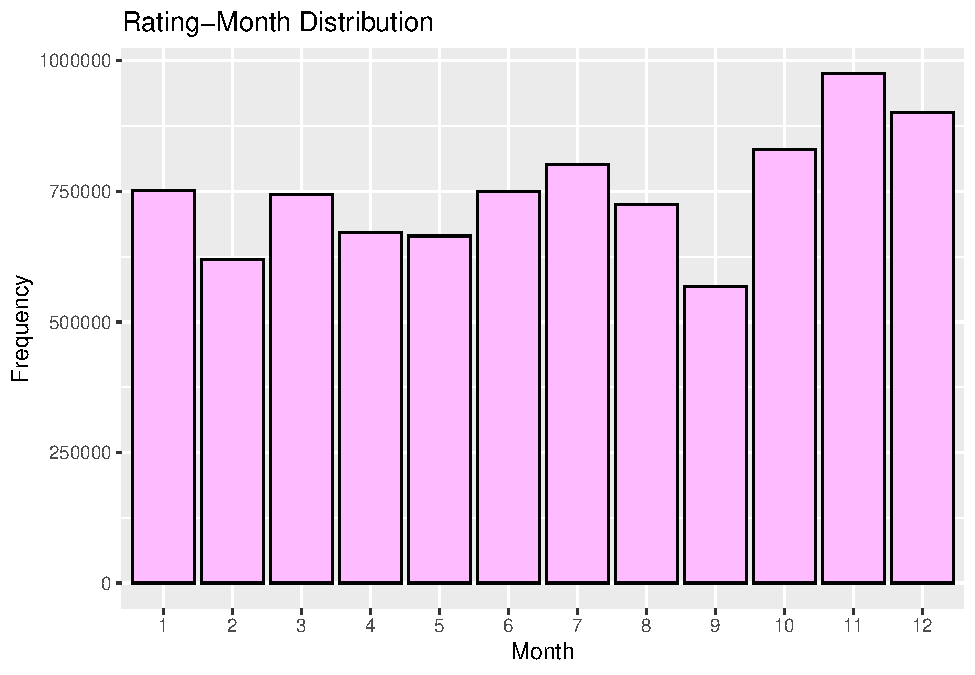
\includegraphics{MovieLens-Report_MitjaPrah_files/figure-latex/unnamed-chunk-24-1} \end{center}

The plot shows that ratings are distributed by months quite evenly.
February and September have slightly lower number of ratings, and the
most movies are rated at the end of year, in November and December.

\newpage

\textbf{Distribution of Number of Ratings per Release Year}

\begin{center}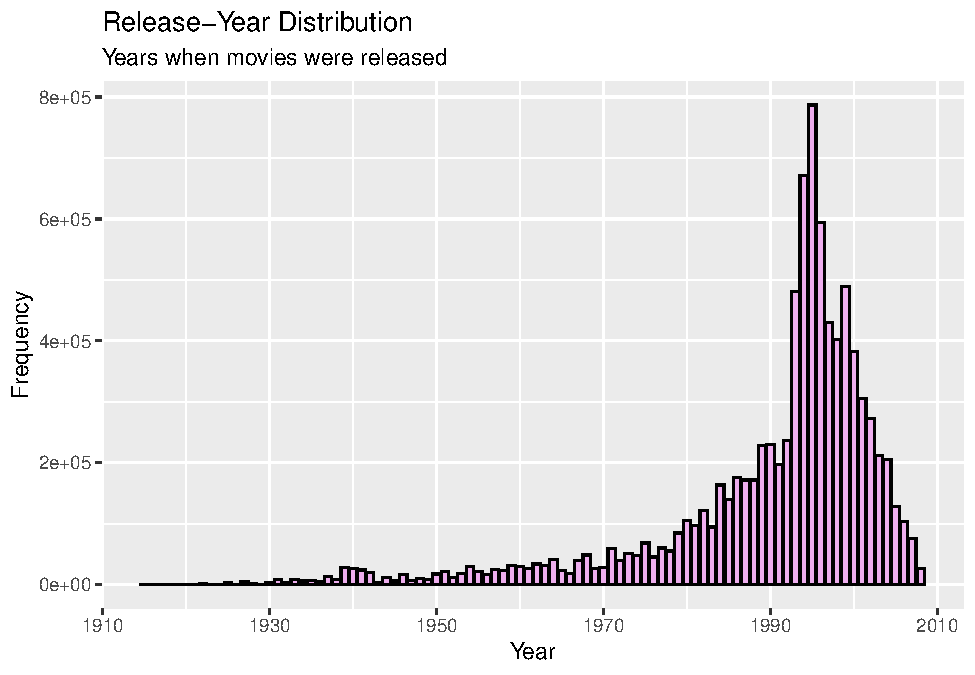
\includegraphics{MovieLens-Report_MitjaPrah_files/figure-latex/unnamed-chunk-25-1} \end{center}

The above plot also clearly shows the left-skewed distribution, which
implies that newer movies, released after 1989, are rated more
frequently than older movies. \textbf{This confirms our initial
assumption of a strong time bias.}

\newpage

\textbf{Distribution of Rating Frequency per Movie}

\begin{center}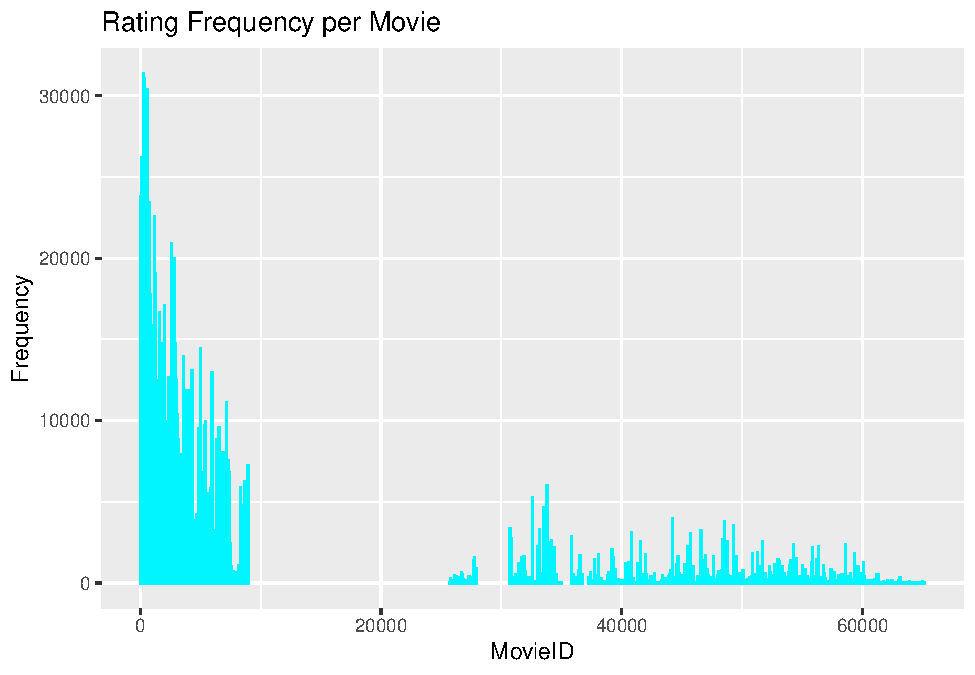
\includegraphics{MovieLens-Report_MitjaPrah_files/figure-latex/unnamed-chunk-26-1} \end{center}

The above plot shows that some movies get rated much more frequently
than others, which is not surprising, given that there are blockbusters
watched by millions and artsy independent movies watched by just a few.
\textbf{This confirms our initial assumption of a strong movie bias.}
The plot also shows that lower movieIds have much higher ratings than
higher movieIds, and there are no movies with movieId between 9,500 and
25,000. Both of these findings are probably due to the system of
clasification used for primary construction of the MovieLens dataset,
and will unlikely affect the model performance.

\newpage

\textbf{Distribution of Rating Frequency per Genre (in the
edx\_test\_split\_genres dataset)}

\begin{center}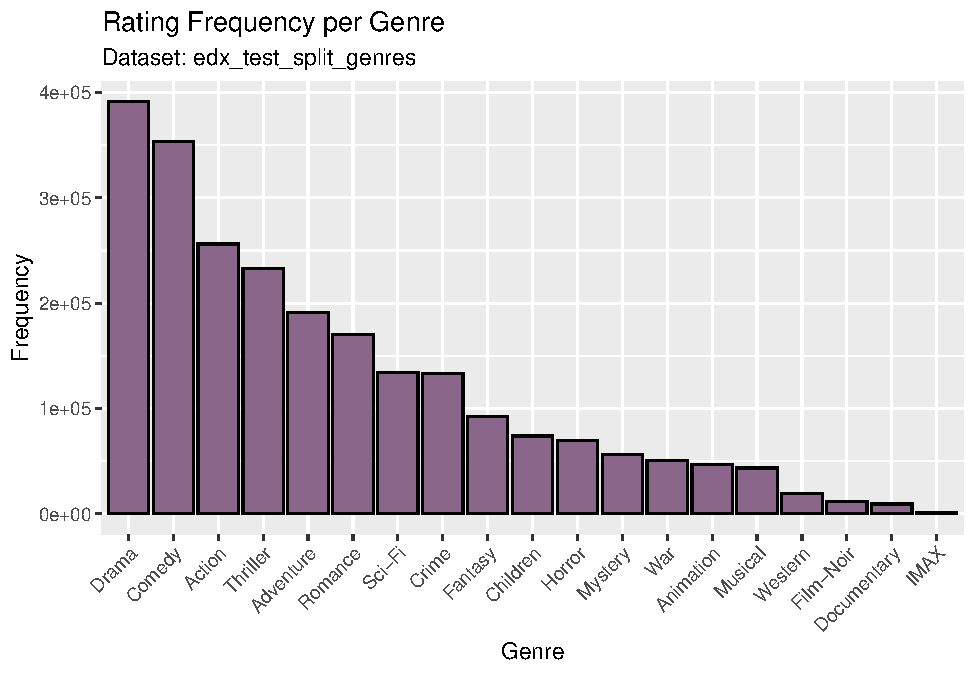
\includegraphics{MovieLens-Report_MitjaPrah_files/figure-latex/unnamed-chunk-28-1} \end{center}

The above plot shows that rating frequency also varies by the movie
genre. \textbf{This confirms our initial assumption of a strong genre
bias.} The most rated (= the most popular) movie genres are Drama and
Comedy, the least rated are Documentary and IMAX. Given the relatively
high number of observations in this dataset, we can assume that this
distribution is similar in the edx dataset.

\newpage

\textbf{Genre Popularity per Rating Year (in the
edx\_test\_split\_genres dataset)}

\begin{center}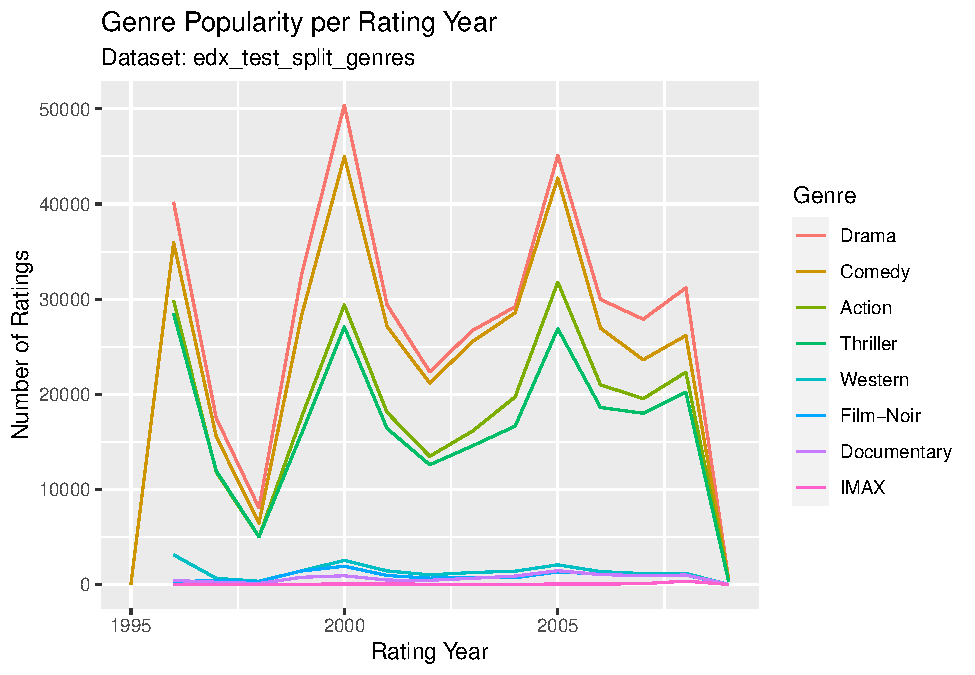
\includegraphics{MovieLens-Report_MitjaPrah_files/figure-latex/unnamed-chunk-29-1} \end{center}

The above plot shows similar year-by-year variability between genres.
For readability, only four the most rated and four the least rated movie
genres are included in the plot.

\newpage

\textbf{Rating Distribution per Users}

\begin{center}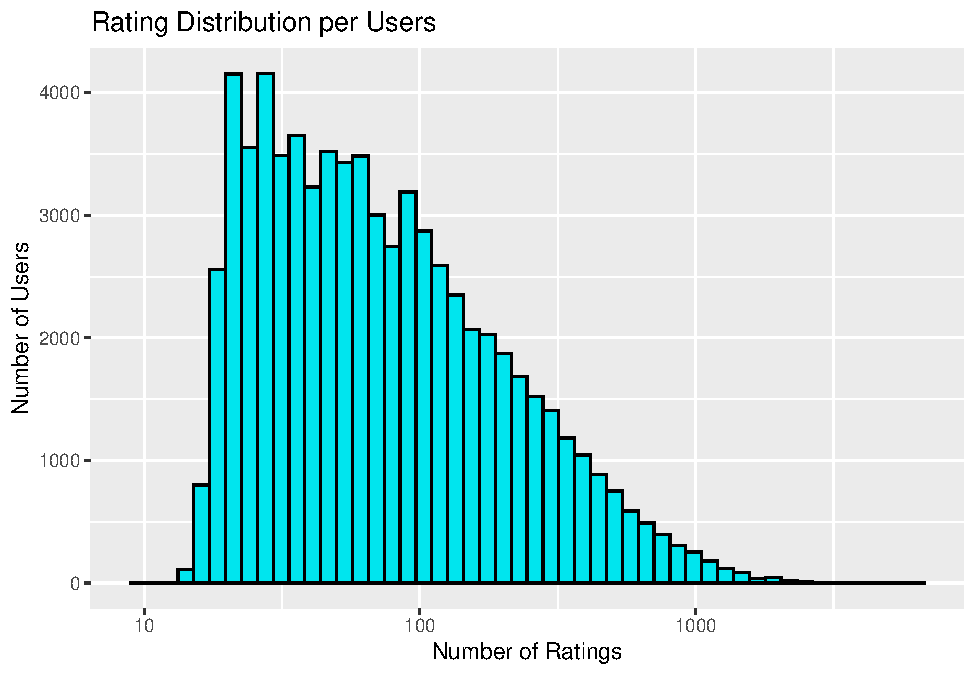
\includegraphics{MovieLens-Report_MitjaPrah_files/figure-latex/unnamed-chunk-30-1} \end{center}

The above plot shows that some users are more active than others. Some
users have rated more than 1000 movies, while the majority have rated
less than 100 movies, and some of them only a handful. \textbf{This
confirms our initial assumption of a strong user bias.}

\newpage

\hypertarget{further-data-exploration---top-ratings}{%
\subsubsection{Further Data Exploration - Top
Ratings}\label{further-data-exploration---top-ratings}}

\textbf{15 Top Rated Movies According To The Number of Ratings}

\begin{center}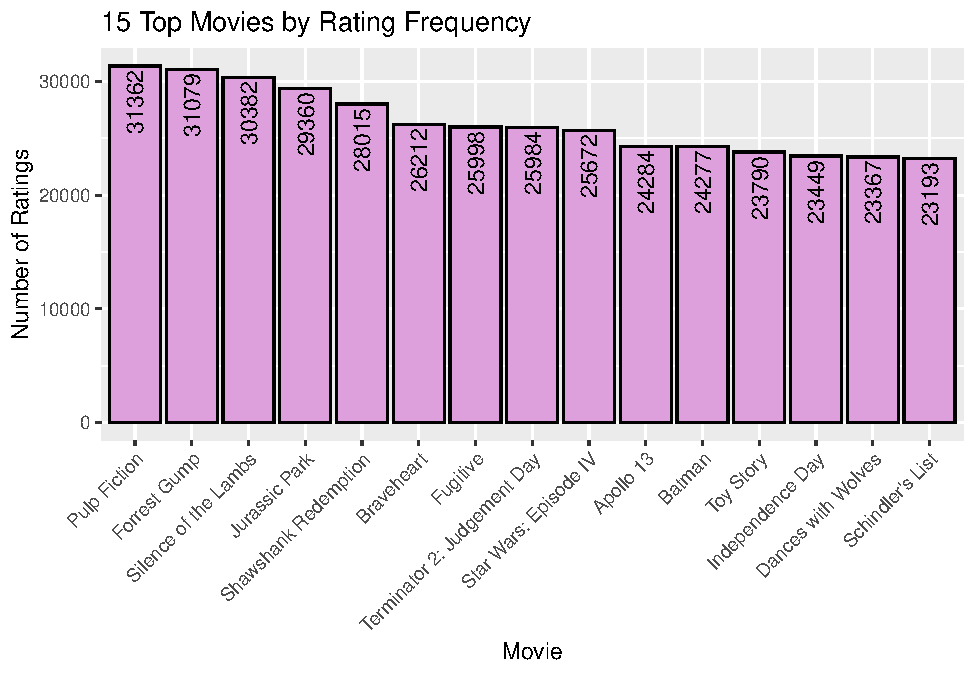
\includegraphics{MovieLens-Report_MitjaPrah_files/figure-latex/unnamed-chunk-31-1} \end{center}

The plot shows 15 most popular movies based on the rating frequency. All
of these movies were rated more than 23,000 times and are well-known
blockbusters.

\newpage

\textbf{15 Top Rated Movies According To The Mean Star Rating}

\begin{center}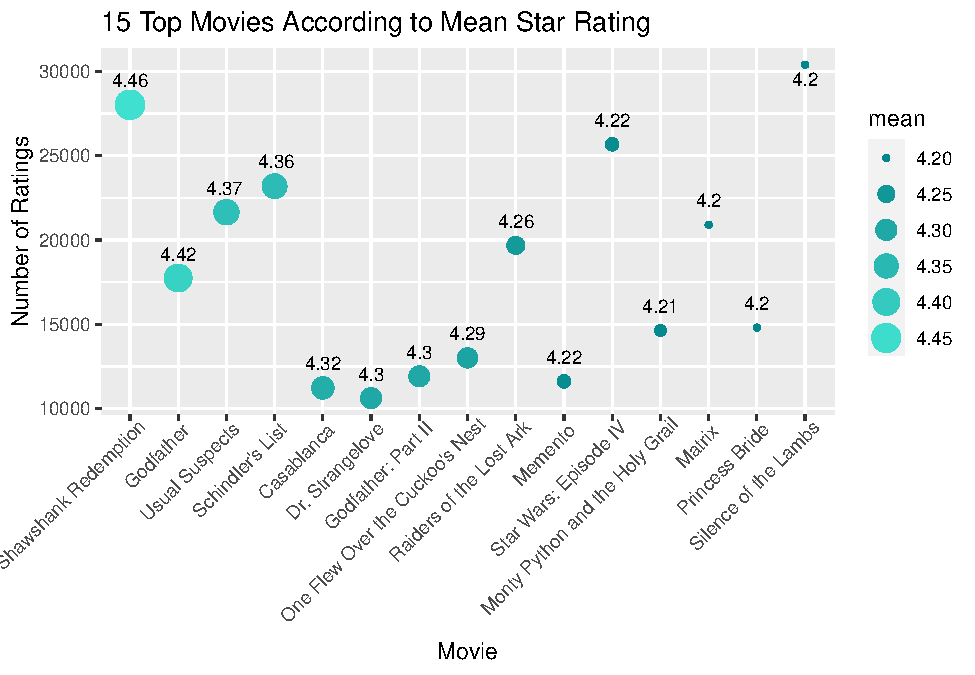
\includegraphics{MovieLens-Report_MitjaPrah_files/figure-latex/unnamed-chunk-32-1} \end{center}

This plot shows 15 most popular movies based on the mean star rating.
Please note that only movies with over 10,000 ratings were included in
this exploratory analysis. Only 4 of these movies are also among the top
15 per rating frequency. All of these are well-known critically
acclaimed movies, as well.

\hypertarget{data-analysis---model-building-and-evaluation}{%
\subsection{Data Analysis - Model Building and
Evaluation}\label{data-analysis---model-building-and-evaluation}}

We will build several models and evaluate them with the RMSE, as already
mentioned earlier. The lower RMSE indicates the better performance of an
individual model. We will focus on the approach called regularization.

\hypertarget{naive-model}{%
\subsubsection{Naive Model}\label{naive-model}}

This is the simplest possible model that always predicts the sample mean
rating across all movies and all users, with all the differences
explained by random variation.

The formula used for this model is:

\[Y_{u,i} = \mu + \varepsilon_{u,i}\]

where \(Y_{u,i}\) is the rating for movie \(i\) by user \(u\), \(\mu\)
is the true sample mean rating and \(\varepsilon_{i,u}\) are independent
errors sampled from the same distribution centered at 0.

\begin{verbatim}
## [1] "The sample mean is: 3.51"
\end{verbatim}

\begin{verbatim}
## [1] "The Naive Model RMSE evaluated on the edx_test dataset is: 1.06005"
\end{verbatim}

\begin{longtable}[]{@{}lr@{}}
\caption{Naive Model RMSE}\tabularnewline
\toprule
Model & RMSE\tabularnewline
\midrule
\endfirsthead
\toprule
Model & RMSE\tabularnewline
\midrule
\endhead
Naive Model & 1.06005\tabularnewline
\bottomrule
\end{longtable}

The above table shows the RMSE value of the simplest model, which we
will try to improve (decrease) with more sophisticated models.

\hypertarget{movie-effect-model}{%
\subsubsection{Movie Effect Model}\label{movie-effect-model}}

To incorporate \emph{movie bias}, shown in the Data Visualization
section, into the existing naive model, we will modify the model
formula:

\[Y_{u,i} = \mu + b_i + \epsilon_{u,i}\]

where the added \(b_i\) represents the average rating for movie \(i\),
i.e.~the bias of a movie \(i\).

The linear model could be used, but would be very slow and could
possibly crash the computer. We will use a simplified approach instead.
In this particular situation, we know that the least square estimate
\(\hat{b_i}\) is just the average of \(Y_{u,i} - \hat{\mu}\) for each
movie \(i\). So we can compute them this way:

\begin{verbatim}
## [1] "The Movie Effect Model RMSE evaluated on the edx_test dataset is: 0.94296"
\end{verbatim}

With the augmented model, we have achieved 10\% drop in RMSE. Therefore,
it seems reasonable to develop this approach further.

\hypertarget{movie-and-user-effect-model}{%
\subsubsection{Movie and User Effect
Model}\label{movie-and-user-effect-model}}

To add \emph{user bias}, shown in the Data Visualization section, into
the existing Movie Effect model, we modify the model formula:

\[Y_{u,i} = \mu + b_i + b_u + \epsilon_{u,i}\]

where the added \(b_u\) represents the average rating for user \(u\),
i.e.~the bias of a user \(u\).

As for the previous model, we use the simplified approach, where the
\(b_u\) is calculated in the following way:

\begin{verbatim}
## [1] "The Movie and User Effect Model RMSE evaluated on the edx_test dataset is: 0.86468"
\end{verbatim}

An additional improvement in the RMSE of more than 5\% was achieved by
adding the user effect. The regularization techniques may improve the
result even further.

\hypertarget{regularization-models-motivated-by-the-netflix-challenge}{%
\subsubsection{Regularization Models (Motivated by the Netflix
Challenge)}\label{regularization-models-motivated-by-the-netflix-challenge}}

Some movies are rated by very few users. With just a few users, we have
more uncertainty. Therefore, larger estimates of \(b_i\), negative or
positive, are more likely.

We can check which are the best and the worst 10 movies according to our
\(b_i\) estimate from the Movie Effect Model in the above section.

\begin{longtable}[]{@{}lr@{}}
\caption{Ten Best Movies by b\_i}\tabularnewline
\toprule
Movie Title & b\_i\tabularnewline
\midrule
\endfirsthead
\toprule
Movie Title & b\_i\tabularnewline
\midrule
\endhead
Hellhounds on My Trail (1999) & 1.487544\tabularnewline
Satan's Tango (Sátántangó) (1994) & 1.487544\tabularnewline
Shadows of Forgotten Ancestors (1964) & 1.487544\tabularnewline
Fighting Elegy (Kenka erejii) (1966) & 1.487544\tabularnewline
Sun Alley (Sonnenallee) (1999) & 1.487544\tabularnewline
Blue Light, The (Das Blaue Licht) (1932) & 1.487544\tabularnewline
Who's Singin' Over There? (a.k.a. Who Sings Over There) (Ko to tamo
peva) (1980) & 1.237544\tabularnewline
Life of Oharu, The (Saikaku ichidai onna) (1952) &
1.237544\tabularnewline
Human Condition II, The (Ningen no joken II) (1959) &
1.237544\tabularnewline
Human Condition III, The (Ningen no joken III) (1961) &
1.237544\tabularnewline
\bottomrule
\end{longtable}

\begin{longtable}[]{@{}lr@{}}
\caption{Ten Worst Movies by b\_i}\tabularnewline
\toprule
Movie Title & b\_i\tabularnewline
\midrule
\endfirsthead
\toprule
Movie Title & b\_i\tabularnewline
\midrule
\endhead
Besotted (2001) & -3.012456\tabularnewline
Hi-Line, The (1999) & -3.012456\tabularnewline
Accused (Anklaget) (2005) & -3.012456\tabularnewline
Confessions of a Superhero (2007) & -3.012456\tabularnewline
War of the Worlds 2: The Next Wave (2008) & -3.012456\tabularnewline
SuperBabies: Baby Geniuses 2 (2004) & -2.767775\tabularnewline
Disaster Movie (2008) & -2.745789\tabularnewline
From Justin to Kelly (2003) & -2.638139\tabularnewline
Hip Hop Witch, Da (2000) & -2.603365\tabularnewline
Criminals (1996) & -2.512456\tabularnewline
\bottomrule
\end{longtable}

They all seem to be quite obscure. Let's look at how often they are
rated.

\begin{longtable}[]{@{}lrr@{}}
\caption{Number of Ratings for Ten Best Movies by b\_i}\tabularnewline
\toprule
Movie Title & b\_i & n\tabularnewline
\midrule
\endfirsthead
\toprule
Movie Title & b\_i & n\tabularnewline
\midrule
\endhead
Hellhounds on My Trail (1999) & 1.487544 & 1\tabularnewline
Satan's Tango (Sátántangó) (1994) & 1.487544 & 1\tabularnewline
Shadows of Forgotten Ancestors (1964) & 1.487544 & 1\tabularnewline
Fighting Elegy (Kenka erejii) (1966) & 1.487544 & 1\tabularnewline
Sun Alley (Sonnenallee) (1999) & 1.487544 & 1\tabularnewline
Blue Light, The (Das Blaue Licht) (1932) & 1.487544 & 1\tabularnewline
Who's Singin' Over There? (a.k.a. Who Sings Over There) (Ko to tamo
peva) (1980) & 1.237544 & 4\tabularnewline
Life of Oharu, The (Saikaku ichidai onna) (1952) & 1.237544 &
2\tabularnewline
Human Condition II, The (Ningen no joken II) (1959) & 1.237544 &
4\tabularnewline
Human Condition III, The (Ningen no joken III) (1961) & 1.237544 &
4\tabularnewline
\bottomrule
\end{longtable}

\begin{longtable}[]{@{}lrr@{}}
\caption{Number of Ratings for Ten Worst Movies by b\_i}\tabularnewline
\toprule
Movie Title & b\_i & n\tabularnewline
\midrule
\endfirsthead
\toprule
Movie Title & b\_i & n\tabularnewline
\midrule
\endhead
Besotted (2001) & -3.012456 & 1\tabularnewline
Hi-Line, The (1999) & -3.012456 & 1\tabularnewline
Accused (Anklaget) (2005) & -3.012456 & 1\tabularnewline
Confessions of a Superhero (2007) & -3.012456 & 1\tabularnewline
War of the Worlds 2: The Next Wave (2008) & -3.012456 & 2\tabularnewline
SuperBabies: Baby Geniuses 2 (2004) & -2.767775 & 47\tabularnewline
Disaster Movie (2008) & -2.745789 & 30\tabularnewline
From Justin to Kelly (2003) & -2.638139 & 183\tabularnewline
Hip Hop Witch, Da (2000) & -2.603365 & 11\tabularnewline
Criminals (1996) & -2.512456 & 1\tabularnewline
\bottomrule
\end{longtable}

The supposed best and worst movies were rated by very few users. These
are noisy estimates that we should not trust, especially when it comes
to prediction. Large errors can increase our RMSE, so we would rather be
conservative when unsure.

Regularization permits us to penalize large estimates that are formed
using small sample sizes. With this it helps us in reducing the effect
of overfitting. The general idea is to add a penalty for large values of
\(b\) to the sum of squares equations.

\hypertarget{regularized-movie-effect-model}{%
\paragraph{Regularized Movie Effect
Model}\label{regularized-movie-effect-model}}

To build a Regularized Movie Effect Model, we minimize the following
equation that adds a penalty:

\[\frac{1}{N} \sum_{u,i} (y_{u,i} - \mu - b_{i})^{2} + \lambda \sum_{i} b_{i}^2\]

The first term is just least squares and the second is a penalty that
gets larger when many \(b_i\) are large. The values of \(b\) that
minimize this equation are given by:

\[\hat{b_{i}} (\lambda) = \frac{1}{\lambda + n_{i}} \sum_{u=1}^{n_{i}} (Y_{u,i} - \hat{\mu}) \]

where \(n_i\) is a number of ratings \(b\) for movie \(i\). The larger
\(\lambda\) is, the more we shrink the \(b_i\), closer to zero.
\(\lambda\) is a tuning parameter, so we can use cross-validation on the
edx\_train dataset to choose it.

\begin{center}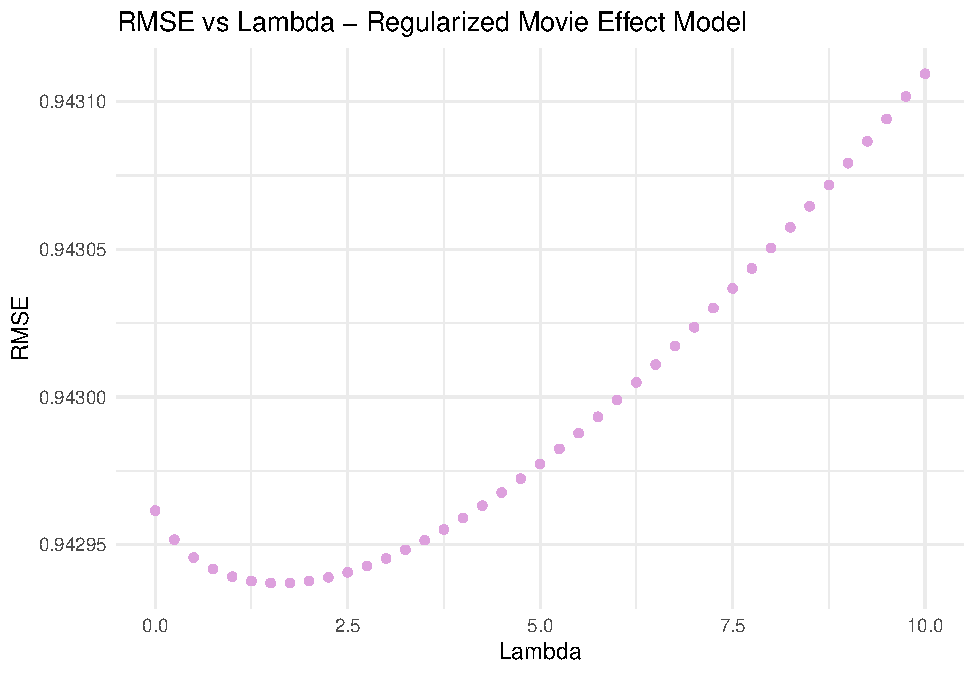
\includegraphics{MovieLens-Report_MitjaPrah_files/figure-latex/unnamed-chunk-43-1} \end{center}

\begin{verbatim}
## [1] "The optimal lambda that minimizes RMSE the most is: 1.5"
\end{verbatim}

\begin{verbatim}
## [1] "The Regularized Movie Effect Model RMSE evaluated on the edx_test dataset is: 0.943"
\end{verbatim}

Unfortunately, the regularized movie effect model yields no improvement
in comparison with the initial movie effect model. However, let's look
at the top 10 best movies based on the penalized estimate
\(\hat{b_{i}} (\lambda)\).

\begin{longtable}[]{@{}lrr@{}}
\caption{Ten Best Movies by b\_i (Regularized Movie Effect
Model)}\tabularnewline
\toprule
Movie Title & b\_i & n\tabularnewline
\midrule
\endfirsthead
\toprule
Movie Title & b\_i & n\tabularnewline
\midrule
\endhead
Shawshank Redemption, The (1994) & 0.9440548 & 25188\tabularnewline
More (1998) & 0.9233688 & 6\tabularnewline
Godfather, The (1972) & 0.9041105 & 15975\tabularnewline
Who's Singin' Over There? (a.k.a. Who Sings Over There) (Ko to tamo
peva) (1980) & 0.9000323 & 4\tabularnewline
Human Condition II, The (Ningen no joken II) (1959) & 0.9000323 &
4\tabularnewline
Human Condition III, The (Ningen no joken III) (1961) & 0.9000323 &
4\tabularnewline
Usual Suspects, The (1995) & 0.8540304 & 19457\tabularnewline
Schindler's List (1993) & 0.8515681 & 20877\tabularnewline
Rear Window (1954) & 0.8123204 & 7115\tabularnewline
Casablanca (1942) & 0.8070680 & 10141\tabularnewline
\bottomrule
\end{longtable}

This makes more sense, as the majority of the listed movies are
well-known blockbusters with high number of ratings. This indicates that
the regularized model is more reliable than the initial, unregularized,
movie effect model.

\begin{longtable}[]{@{}lrr@{}}
\caption{Ten Worst Movies by b\_i (Regularized Movie Effect
Model)}\tabularnewline
\toprule
Movie Title & b\_i & n\tabularnewline
\midrule
\endfirsthead
\toprule
Movie Title & b\_i & n\tabularnewline
\midrule
\endhead
SuperBabies: Baby Geniuses 2 (2004) & -2.682174 & 47\tabularnewline
From Justin to Kelly (2003) & -2.616690 & 183\tabularnewline
Disaster Movie (2008) & -2.615037 & 30\tabularnewline
Pokémon Heroes (2003) & -2.442586 & 124\tabularnewline
Barney's Great Adventure (1998) & -2.353689 & 186\tabularnewline
Carnosaur 3: Primal Species (1996) & -2.340157 & 61\tabularnewline
Glitter (2001) & -2.327596 & 311\tabularnewline
Gigli (2003) & -2.302655 & 281\tabularnewline
Pokemon 4 Ever (a.k.a. Pokémon 4: The Movie) (2002) & -2.292040 &
188\tabularnewline
Hip Hop Witch, Da (2000) & -2.290961 & 11\tabularnewline
\bottomrule
\end{longtable}

Similarly, a look at the 10 worst movies according to the Regularized
Movie Effect model reveals differences when compared to the output of
the unregularized movie effect model.

\hypertarget{regularized-movie-and-user-effect-model}{%
\paragraph{Regularized Movie and User Effect
Model}\label{regularized-movie-and-user-effect-model}}

Additional regularization for the estimated user effects could yield
further improvement in the RMSE reduction. We are minimizing the
following equation:

\[\frac{1}{N} \sum_{u,i} (y_{u,i} - \mu - b_{i} - b_{u})^{2} + \lambda (\sum_{i} b_{i}^2 + \sum_{u} b_{u}^2)\]

\begin{center}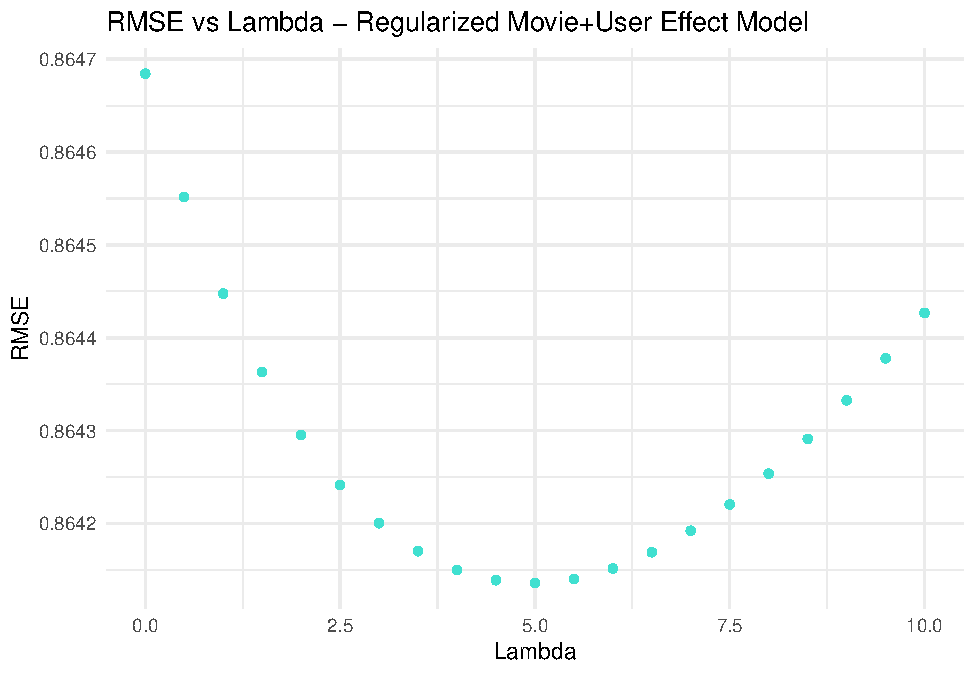
\includegraphics{MovieLens-Report_MitjaPrah_files/figure-latex/unnamed-chunk-47-1} \end{center}

The optimal lambda that minimizes RMSE in the Regularized Movie And User
Effect Model the most is:

\begin{verbatim}
## [1] "5"
\end{verbatim}

The Regularized Movie And User Effect Model RMSE, evaluated on the
edx\_test dataset is:

\begin{verbatim}
## [1] "0.86428"
\end{verbatim}

The regularized movie and user effect model provided a minimal, but
important improvement in the RMSE, when compared to the unregularized
movie and user effect model. It is the most accurate model so far.

\hypertarget{regularized-movie-and-user-and-genre-and-time-effect-model}{%
\paragraph{Regularized Movie and User and Genre and Time Effect
Model}\label{regularized-movie-and-user-and-genre-and-time-effect-model}}

Finally, we will incorporate the effects of genre bias and time bias in
the latter model. The equation we are minimizing is:

\[\frac{1}{N} \sum_{u,i} (y_{u,i} - \mu - b_{i} - b_{u} - b_{g} - b_{t})^{2} + \lambda (\sum_{i} b_{i}^2 + \sum_{u} b_{u}^2 + \sum_{g} b_{g}^2 + \sum_{t} b_{t}^2)\]

Please note that due to limited computer memory capacity, mentioned in
previous sections, the \emph{genres} variable from the edx\_train
dataset is left unsplit (i.e.~composed of several genres that describe
an individual movie). Ideally, this variable would be split into
individual genres, in the same manner as it was done in the
edx\_test\_split\_genres dataset, which was used to explore the genre
bias in the sections \emph{Distribution of Rating Frequency per Genre
(in the edx\_test\_split\_genres dataset)} and \emph{Genre Popularity
per Rating Year (in the edx\_test\_split\_genres dataset)}.\\
For time bias effect, the \emph{year\_release} variable is used.

\begin{center}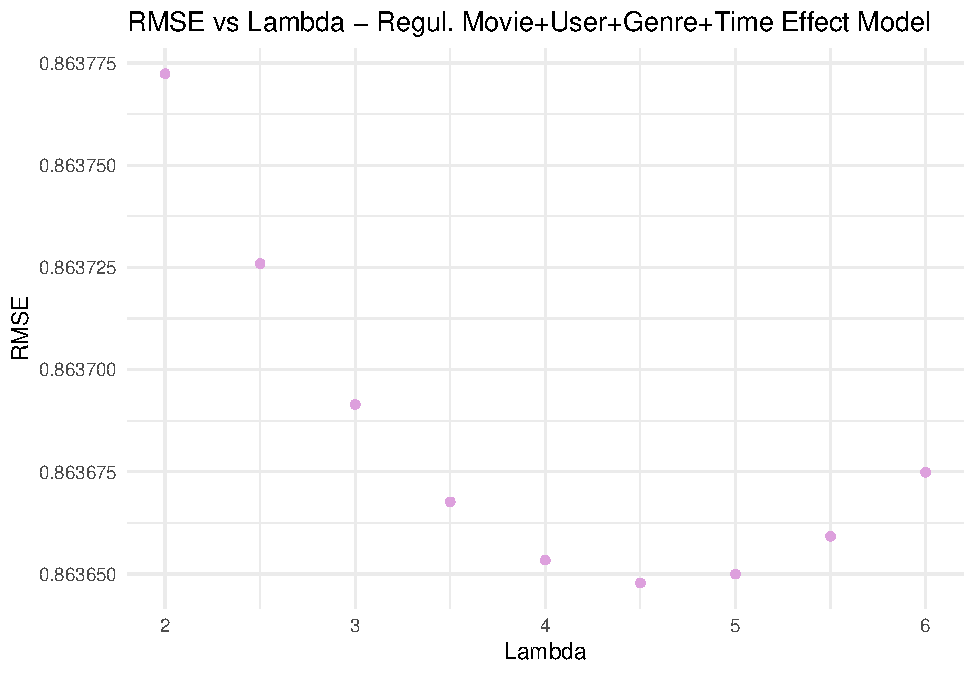
\includegraphics{MovieLens-Report_MitjaPrah_files/figure-latex/unnamed-chunk-51-1} \end{center}

The optimal lambda that minimizes RMSE in the Regularized
Movie+User+Genre+Time Effect Model the most is:

\begin{verbatim}
## [1] "4.5"
\end{verbatim}

The Regularized Movie+User+Genre+Time Effect Model RMSE, evaluated on
the edx\_test dataset is:

\begin{verbatim}
## [1] "0.86368"
\end{verbatim}

As anticipated, the regularized model combining all four types of major
biases is the most accurate, i.e.~yields the lowest RMSE. Therefore,
this model is selected as our final model to be tested on the
\emph{validation} dataset.

\newpage

\hypertarget{results}{%
\section{Results}\label{results}}

\hypertarget{combined-results-of-all-models}{%
\subsection{Combined results of all
models}\label{combined-results-of-all-models}}

The following table shows the results of all the models trained on
edx\_train dataset and evaluated on edx\_test dataset:

\begin{longtable}[]{@{}lr@{}}
\caption{RMSEs of All Models}\tabularnewline
\toprule
Model & RMSE\tabularnewline
\midrule
\endfirsthead
\toprule
Model & RMSE\tabularnewline
\midrule
\endhead
Naive Model & 1.06005\tabularnewline
Movie Effect Model & 0.94296\tabularnewline
Movie+User Effect Model & 0.86468\tabularnewline
Regularized Movie Effect Model & 0.94300\tabularnewline
Regularized Movie+User Effect Model & 0.86428\tabularnewline
Regularized Movie+User+Genre+Time Effect Model & 0.86368\tabularnewline
\bottomrule
\end{longtable}

\hypertarget{the-final-model-evaluation-on-the-validation-dataset}{%
\subsection{The Final Model Evaluation on The Validation
Dataset}\label{the-final-model-evaluation-on-the-validation-dataset}}

Finally, the selected best model is tested on the \textbf{validation
dataset}. The result is presented in the following table.

\begin{longtable}[]{@{}lr@{}}
\caption{Final Model RMSE on Validation Dataset}\tabularnewline
\toprule
Final Model & RMSE on Validation Set\tabularnewline
\midrule
\endfirsthead
\toprule
Final Model & RMSE on Validation Set\tabularnewline
\midrule
\endhead
Regularized Movie+User+Genre+Time Effect Model & 0.86429\tabularnewline
\bottomrule
\end{longtable}

\newpage

\hypertarget{conclusion}{%
\section{Conclusion}\label{conclusion}}

Through building several models, we observed gradual lowering of the
Root Mean Squared Error (RMSE), which was predefined as our \emph{loss
function}. As expected, the simplest, baseline naive model, that always
predicts the sample mean rating across all movies and all users,
performed the worst. After introducing the movie effect and the user
effect into the naive model, we achieved a substantial decrease in the
RMSE of 11\% and further 8\%, respectively. By the use of the
regularization method we were able to slightly lower the RMSE even
further. The introduction of the genre effect and the time effect caused
a minor, but not negligible, additional decrease in the RMSE.\\
The regularized model combining all four types of the major biases
yielded the lowest RMSE, and was therefore selected as the final, the
optimal model.

With the selected final model, that we subsequently tested on the
\emph{validation} dataset, we were able to achieve and improve the
target RMSE of \textbf{\textless0.86490}, which is a great result given
the simplicity of the model. Hence, we can conclude that the primary
objective of this project was reached.

The final model could potentially be slightly improved even further, if
the combined \emph{genres} variable would be split into individual
genres. However, as discussed in the body of the report, such splitting
was not feasible in this project due to computer-memory limitations.

In future efforts, a model based on matrix factorization technique could
be tried, since it can potentionally achieve even higher accuracy with
additional improvements in the lowering of the RMSE.

\hypertarget{references}{%
\section{References}\label{references}}

\begin{enumerate}
\def\labelenumi{\arabic{enumi}.}
\tightlist
\item
  Irizarry RA. Introduction to Data Science: Data Analysis and
  Prediction Algorithms with R: CRC Press; 2019.
\item
  \url{https://github.com/AlessandroCorradini/Harvard-Data-Science-Professional/tree/master/09\%20-\%20PH125.9x\%20-\%20Capstone/MovieLens\%20Recommender\%20System\%20Project}
\item
  \url{https://www.rpubs.com/rezapci/MovieLens}
\end{enumerate}

\newpage

\hypertarget{appendices}{%
\section{Appendices}\label{appendices}}

\hypertarget{code-previously-provided-by-edx}{%
\subsection{Code Previously Provided by
edX}\label{code-previously-provided-by-edx}}

\begin{Shaded}
\begin{Highlighting}[]
\CommentTok{###SCRIPT - Pre-provided code}
\CommentTok{#The following code for generating datasets was provided in the course:}
\CommentTok{##########################################################}
\CommentTok{# Create edx set, validation set (final hold-out test set)}
\CommentTok{##########################################################}

\ControlFlowTok{if}\NormalTok{(}\OperatorTok{!}\KeywordTok{require}\NormalTok{(tidyverse)) }\KeywordTok{install.packages}\NormalTok{(}\StringTok{"tidyverse"}\NormalTok{, }\DataTypeTok{repos =} \StringTok{"http://cran.us.r-project.org"}\NormalTok{)}
\ControlFlowTok{if}\NormalTok{(}\OperatorTok{!}\KeywordTok{require}\NormalTok{(caret)) }\KeywordTok{install.packages}\NormalTok{(}\StringTok{"caret"}\NormalTok{, }\DataTypeTok{repos =} \StringTok{"http://cran.us.r-project.org"}\NormalTok{)}
\ControlFlowTok{if}\NormalTok{(}\OperatorTok{!}\KeywordTok{require}\NormalTok{(data.table)) }\KeywordTok{install.packages}\NormalTok{(}\StringTok{"data.table"}\NormalTok{, }\DataTypeTok{repos =} \StringTok{"http://cran.us.r-project.org"}\NormalTok{)}

\KeywordTok{library}\NormalTok{(tidyverse)}
\KeywordTok{library}\NormalTok{(caret)}
\KeywordTok{library}\NormalTok{(data.table)}

\CommentTok{# MovieLens 10M dataset:}
\CommentTok{# https://grouplens.org/datasets/movielens/10m/}
\CommentTok{# http://files.grouplens.org/datasets/movielens/ml-10m.zip}

\NormalTok{dl <-}\StringTok{ }\KeywordTok{tempfile}\NormalTok{()}
\KeywordTok{download.file}\NormalTok{(}\StringTok{"http://files.grouplens.org/datasets/movielens/ml-10m.zip"}\NormalTok{, dl)}

\NormalTok{ratings <-}\StringTok{ }\KeywordTok{fread}\NormalTok{(}\DataTypeTok{text =} \KeywordTok{gsub}\NormalTok{(}\StringTok{"::"}\NormalTok{, }\StringTok{"}\CharTok{\textbackslash{}t}\StringTok{"}\NormalTok{, }\KeywordTok{readLines}\NormalTok{(}\KeywordTok{unzip}\NormalTok{(dl, }\StringTok{"ml-10M100K/ratings.dat"}\NormalTok{))),}
                 \DataTypeTok{col.names =} \KeywordTok{c}\NormalTok{(}\StringTok{"userId"}\NormalTok{, }\StringTok{"movieId"}\NormalTok{, }\StringTok{"rating"}\NormalTok{, }\StringTok{"timestamp"}\NormalTok{))}

\NormalTok{movies <-}\StringTok{ }\KeywordTok{str_split_fixed}\NormalTok{(}\KeywordTok{readLines}\NormalTok{(}\KeywordTok{unzip}\NormalTok{(dl, }\StringTok{"ml-10M100K/movies.dat"}\NormalTok{)), }\StringTok{"}\CharTok{\textbackslash{}\textbackslash{}}\StringTok{::"}\NormalTok{, }\DecValTok{3}\NormalTok{)}
\KeywordTok{colnames}\NormalTok{(movies) <-}\StringTok{ }\KeywordTok{c}\NormalTok{(}\StringTok{"movieId"}\NormalTok{, }\StringTok{"title"}\NormalTok{, }\StringTok{"genres"}\NormalTok{)}

\CommentTok{# if using R 3.6 or earlier:}
\NormalTok{movies <-}\StringTok{ }\KeywordTok{as.data.frame}\NormalTok{(movies) }\OperatorTok\StringTok{ }\KeywordTok{mutate}\NormalTok{(}\DataTypeTok{movieId =} \KeywordTok{as.numeric}\NormalTok{(}\KeywordTok{levels}\NormalTok{(movieId))[movieId],}
                                           \DataTypeTok{title =} \KeywordTok{as.character}\NormalTok{(title),}
                                           \DataTypeTok{genres =} \KeywordTok{as.character}\NormalTok{(genres))}
\CommentTok{# if using R 4.0 or later:}
\NormalTok{movies <-}\StringTok{ }\KeywordTok{as.data.frame}\NormalTok{(movies) }\OperatorTok\StringTok{ }\KeywordTok{mutate}\NormalTok{(}\DataTypeTok{movieId =} \KeywordTok{as.numeric}\NormalTok{(movieId),}
                                           \DataTypeTok{title =} \KeywordTok{as.character}\NormalTok{(title),}
                                           \DataTypeTok{genres =} \KeywordTok{as.character}\NormalTok{(genres))}


\NormalTok{movielens <-}\StringTok{ }\KeywordTok{left_join}\NormalTok{(ratings, movies, }\DataTypeTok{by =} \StringTok{"movieId"}\NormalTok{)}

\CommentTok{# Validation set will be 10% of MovieLens data}
\KeywordTok{set.seed}\NormalTok{(}\DecValTok{1}\NormalTok{) }\CommentTok{# if using R 3.5}
\NormalTok{test_index <-}\StringTok{ }\KeywordTok{createDataPartition}\NormalTok{(}\DataTypeTok{y =}\NormalTok{ movielens}\OperatorTok{$}\NormalTok{rating, }\DataTypeTok{times =} \DecValTok{1}\NormalTok{, }\DataTypeTok{p =} \FloatTok{0.1}\NormalTok{, }\DataTypeTok{list =} \OtherTok{FALSE}\NormalTok{)}
\NormalTok{edx <-}\StringTok{ }\NormalTok{movielens[}\OperatorTok{-}\NormalTok{test_index,]}
\NormalTok{temp <-}\StringTok{ }\NormalTok{movielens[test_index,]}

\CommentTok{# Make sure userId and movieId in validation set are also in edx set}
\NormalTok{validation <-}\StringTok{ }\NormalTok{temp }\OperatorTok\StringTok{ }
\StringTok{  }\KeywordTok{semi_join}\NormalTok{(edx, }\DataTypeTok{by =} \StringTok{"movieId"}\NormalTok{) }\OperatorTok
\StringTok{  }\KeywordTok{semi_join}\NormalTok{(edx, }\DataTypeTok{by =} \StringTok{"userId"}\NormalTok{)}

\CommentTok{# Add rows removed from validation set back into edx set}
\NormalTok{removed <-}\StringTok{ }\KeywordTok{anti_join}\NormalTok{(temp, validation)}
\NormalTok{edx <-}\StringTok{ }\KeywordTok{rbind}\NormalTok{(edx, removed)}
\end{Highlighting}
\end{Shaded}

\hypertarget{code-generated-in-this-research-project}{%
\subsection{Code Generated in This Research
Project}\label{code-generated-in-this-research-project}}

\begin{Shaded}
\begin{Highlighting}[]
\CommentTok{###SCRIPT Exploratory Data Analysis}

\CommentTok{#RMSE function:}
\NormalTok{RMSE <-}\StringTok{ }\ControlFlowTok{function}\NormalTok{(true_ratings, predicted_ratings)\{}
  \KeywordTok{sqrt}\NormalTok{(}\KeywordTok{mean}\NormalTok{((true_ratings }\OperatorTok{-}\StringTok{ }\NormalTok{predicted_ratings)}\OperatorTok{^}\DecValTok{2}\NormalTok{))}
\NormalTok{\}}

\CommentTok{# Install other needed libraries if not already present}
\ControlFlowTok{if}\NormalTok{(}\OperatorTok{!}\KeywordTok{require}\NormalTok{(kableExtra)) }\KeywordTok{install.packages}\NormalTok{(}\StringTok{"kableExtra"}\NormalTok{)}

\CommentTok{# Loading other needed libraries}
\KeywordTok{library}\NormalTok{(kableExtra)}

\CommentTok{#Split the edx dataset into edx_train and edx_test set.}
\KeywordTok{set.seed}\NormalTok{(}\DecValTok{1}\NormalTok{)}
\NormalTok{test_index1 <-}\StringTok{ }\KeywordTok{createDataPartition}\NormalTok{(}\DataTypeTok{y =}\NormalTok{ edx}\OperatorTok{$}\NormalTok{rating, }\DataTypeTok{times =} \DecValTok{1}\NormalTok{, }\DataTypeTok{p =} \FloatTok{0.1}\NormalTok{, }\DataTypeTok{list =} \OtherTok{FALSE}\NormalTok{)}
\NormalTok{edx_train <-}\StringTok{ }\NormalTok{edx[}\OperatorTok{-}\NormalTok{test_index1,]}
\NormalTok{temp1 <-}\StringTok{ }\NormalTok{edx[test_index1,]}

\CommentTok{# Make sure userId and movieId in edx_test set are also in edx_train set}
\NormalTok{edx_test <-}\StringTok{ }\NormalTok{temp1 }\OperatorTok\StringTok{ }
\StringTok{  }\KeywordTok{semi_join}\NormalTok{(edx_train, }\DataTypeTok{by =} \StringTok{"movieId"}\NormalTok{) }\OperatorTok
\StringTok{  }\KeywordTok{semi_join}\NormalTok{(edx_train, }\DataTypeTok{by =} \StringTok{"userId"}\NormalTok{)}

\CommentTok{# Add rows removed from validation set back into edx set}
\NormalTok{removed <-}\StringTok{ }\KeywordTok{anti_join}\NormalTok{(temp1, edx_test)}
\NormalTok{edx_train <-}\StringTok{ }\KeywordTok{rbind}\NormalTok{(edx_train, removed)}

\CommentTok{#Observe the edx dataset}
\KeywordTok{str}\NormalTok{(edx)}
\CommentTok{#Check edx for missing values}
\KeywordTok{sum}\NormalTok{(}\KeywordTok{is.na}\NormalTok{(edx))}
\CommentTok{#Determine the number of different users and movies:}
\NormalTok{edx }\OperatorTok\StringTok{ }\KeywordTok{summarise}\NormalTok{(}\DataTypeTok{Users =} \KeywordTok{n_distinct}\NormalTok{(userId), }\DataTypeTok{Movies =} \KeywordTok{n_distinct}\NormalTok{(movieId))}

\CommentTok{#Descriptive statistics of the edx dataset}
\NormalTok{edx }\OperatorTok\StringTok{ }\KeywordTok{summarize}\NormalTok{(}\DataTypeTok{N_users =} \KeywordTok{n_distinct}\NormalTok{(userId), }\DataTypeTok{N_movies =} \KeywordTok{n_distinct}\NormalTok{(movieId),}
                  \DataTypeTok{Mean_rating =} \KeywordTok{mean}\NormalTok{(rating), }\DataTypeTok{Median_rating =} \KeywordTok{median}\NormalTok{(rating),}
                  \DataTypeTok{Min_rating =} \KeywordTok{min}\NormalTok{(rating), }\DataTypeTok{Max_rating =} \KeywordTok{max}\NormalTok{(rating)) }\OperatorTok
\StringTok{  }\KeywordTok{kable}\NormalTok{() }\OperatorTok
\StringTok{  }\KeywordTok{kable_styling}\NormalTok{(}\DataTypeTok{bootstrap_options =} \KeywordTok{c}\NormalTok{(}\StringTok{"striped"}\NormalTok{, }\StringTok{"hover"}\NormalTok{, }\StringTok{"condensed"}\NormalTok{, }\StringTok{"responsive"}\NormalTok{),}
                \DataTypeTok{position =} \StringTok{"center"}\NormalTok{,}
                \DataTypeTok{font_size =} \DecValTok{10}\NormalTok{,}
                \DataTypeTok{full_width =} \OtherTok{FALSE}\NormalTok{)}

\CommentTok{#The first 6 rows of the edx dataset}
\KeywordTok{head}\NormalTok{(edx) }\OperatorTok
\StringTok{  }\KeywordTok{kable}\NormalTok{() }\OperatorTok
\StringTok{  }\KeywordTok{kable_styling}\NormalTok{(}\DataTypeTok{latex_options =} \StringTok{"scale_down"}\NormalTok{,}
                \DataTypeTok{bootstrap_options =} \KeywordTok{c}\NormalTok{(}\StringTok{"striped"}\NormalTok{, }\StringTok{"hover"}\NormalTok{, }\StringTok{"condensed"}\NormalTok{, }\StringTok{"responsive"}\NormalTok{),}
                \DataTypeTok{position =} \StringTok{"center"}\NormalTok{,}
                \DataTypeTok{font_size =} \DecValTok{10}\NormalTok{,}
                \DataTypeTok{full_width =} \OtherTok{FALSE}\NormalTok{)}

\CommentTok{#Observe the edx_train dataset}
\KeywordTok{str}\NormalTok{(edx_train)}
\CommentTok{#Check edx_train for missing values}
\KeywordTok{sum}\NormalTok{(}\KeywordTok{is.na}\NormalTok{(edx_train))}
\CommentTok{#Determine the number of different users and movies:}
\NormalTok{edx_train }\OperatorTok\StringTok{ }\KeywordTok{summarise}\NormalTok{(}\DataTypeTok{Users =} \KeywordTok{n_distinct}\NormalTok{(userId), }\DataTypeTok{Movies =} \KeywordTok{n_distinct}\NormalTok{(movieId))}

\CommentTok{#Observe the edx_test dataset}
\KeywordTok{str}\NormalTok{(edx_test)}
\CommentTok{#Check edx_test for missing values}
\KeywordTok{sum}\NormalTok{(}\KeywordTok{is.na}\NormalTok{(edx_test))}
\CommentTok{#Determine the number of different users and movies:}
\NormalTok{edx_test }\OperatorTok\StringTok{ }\KeywordTok{summarise}\NormalTok{(}\DataTypeTok{Users =} \KeywordTok{n_distinct}\NormalTok{(userId), }\DataTypeTok{Movies =} \KeywordTok{n_distinct}\NormalTok{(movieId))}

\CommentTok{#Observe the validation dataset}
\KeywordTok{str}\NormalTok{(validation)}
\CommentTok{#Check edx for missing values}
\KeywordTok{sum}\NormalTok{(}\KeywordTok{is.na}\NormalTok{(validation))}
\CommentTok{#Determine the number of different users and movies:}
\NormalTok{validation }\OperatorTok\StringTok{ }\KeywordTok{summarise}\NormalTok{(}\DataTypeTok{Users =} \KeywordTok{n_distinct}\NormalTok{(userId), }\DataTypeTok{Movies =} \KeywordTok{n_distinct}\NormalTok{(movieId))}

\CommentTok{##The first 6 rows of the validation dataset}
\KeywordTok{head}\NormalTok{(validation) }\OperatorTok
\StringTok{  }\KeywordTok{kable}\NormalTok{() }\OperatorTok
\StringTok{  }\KeywordTok{kable_styling}\NormalTok{(}\DataTypeTok{latex_options =} \StringTok{"scale_down"}\NormalTok{,}
                \DataTypeTok{bootstrap_options =} \KeywordTok{c}\NormalTok{(}\StringTok{"striped"}\NormalTok{, }\StringTok{"hover"}\NormalTok{, }\StringTok{"condensed"}\NormalTok{, }\StringTok{"responsive"}\NormalTok{),}
                \DataTypeTok{position =} \StringTok{"center"}\NormalTok{,}
                \DataTypeTok{font_size =} \DecValTok{10}\NormalTok{,}
                \DataTypeTok{full_width =} \OtherTok{FALSE}\NormalTok{)}

\CommentTok{#Descriptive statistics of the validation dataset}
\NormalTok{validation }\OperatorTok\StringTok{ }\KeywordTok{summarize}\NormalTok{(}\DataTypeTok{N_users =} \KeywordTok{n_distinct}\NormalTok{(userId), }\DataTypeTok{N_movies =} \KeywordTok{n_distinct}\NormalTok{(movieId),}
                  \DataTypeTok{Mean_rating =} \KeywordTok{mean}\NormalTok{(rating), }\DataTypeTok{Median_rating =} \KeywordTok{median}\NormalTok{(rating),}
                  \DataTypeTok{Min_rating =} \KeywordTok{min}\NormalTok{(rating), }\DataTypeTok{Max_rating =} \KeywordTok{max}\NormalTok{(rating)) }\OperatorTok
\StringTok{  }\KeywordTok{kable}\NormalTok{() }\OperatorTok
\StringTok{  }\KeywordTok{kable_styling}\NormalTok{(}\DataTypeTok{bootstrap_options =} \KeywordTok{c}\NormalTok{(}\StringTok{"striped"}\NormalTok{, }\StringTok{"hover"}\NormalTok{, }\StringTok{"condensed"}\NormalTok{, }\StringTok{"responsive"}\NormalTok{),}
                \DataTypeTok{position =} \StringTok{"center"}\NormalTok{,}
                \DataTypeTok{font_size =} \DecValTok{10}\NormalTok{,}
                \DataTypeTok{full_width =} \OtherTok{FALSE}\NormalTok{)}


\CommentTok{#convert timestamp to a human readable date format}
\NormalTok{edx}\OperatorTok{$}\NormalTok{date <-}\StringTok{ }\KeywordTok{as.POSIXct}\NormalTok{(edx}\OperatorTok{$}\NormalTok{timestamp, }\DataTypeTok{origin=}\StringTok{"1970-01-01"}\NormalTok{)}
\NormalTok{edx_train}\OperatorTok{$}\NormalTok{date <-}\StringTok{ }\KeywordTok{as.POSIXct}\NormalTok{(edx_train}\OperatorTok{$}\NormalTok{timestamp, }\DataTypeTok{origin=}\StringTok{"1970-01-01"}\NormalTok{)}
\NormalTok{edx_test}\OperatorTok{$}\NormalTok{date <-}\StringTok{ }\KeywordTok{as.POSIXct}\NormalTok{(edx_test}\OperatorTok{$}\NormalTok{timestamp, }\DataTypeTok{origin=}\StringTok{"1970-01-01"}\NormalTok{)}
\NormalTok{validation}\OperatorTok{$}\NormalTok{date <-}\StringTok{ }\KeywordTok{as.POSIXct}\NormalTok{(validation}\OperatorTok{$}\NormalTok{timestamp, }\DataTypeTok{origin=}\StringTok{"1970-01-01"}\NormalTok{)}

\CommentTok{#Extract the month and year of the movie rating from the converted timestamp variable}
\NormalTok{edx}\OperatorTok{$}\NormalTok{Rating_Year <-}\StringTok{ }\KeywordTok{format}\NormalTok{(edx}\OperatorTok{$}\NormalTok{date,}\StringTok{"%Y"}\NormalTok{)}
\NormalTok{edx}\OperatorTok{$}\NormalTok{Rating_Month <-}\StringTok{ }\KeywordTok{format}\NormalTok{(edx}\OperatorTok{$}\NormalTok{date,}\StringTok{"%m"}\NormalTok{)}
\NormalTok{edx_train}\OperatorTok{$}\NormalTok{Rating_Year <-}\StringTok{ }\KeywordTok{format}\NormalTok{(edx_train}\OperatorTok{$}\NormalTok{date,}\StringTok{"%Y"}\NormalTok{)}
\NormalTok{edx_train}\OperatorTok{$}\NormalTok{Rating_Month <-}\StringTok{ }\KeywordTok{format}\NormalTok{(edx_train}\OperatorTok{$}\NormalTok{date,}\StringTok{"%m"}\NormalTok{)}
\NormalTok{edx_test}\OperatorTok{$}\NormalTok{Rating_Year <-}\StringTok{ }\KeywordTok{format}\NormalTok{(edx_test}\OperatorTok{$}\NormalTok{date,}\StringTok{"%Y"}\NormalTok{)}
\NormalTok{edx_test}\OperatorTok{$}\NormalTok{Rating_Month <-}\StringTok{ }\KeywordTok{format}\NormalTok{(edx_test}\OperatorTok{$}\NormalTok{date,}\StringTok{"%m"}\NormalTok{)}
\NormalTok{validation}\OperatorTok{$}\NormalTok{Rating_Year <-}\StringTok{ }\KeywordTok{format}\NormalTok{(validation}\OperatorTok{$}\NormalTok{date,}\StringTok{"%Y"}\NormalTok{)}
\NormalTok{validation}\OperatorTok{$}\NormalTok{Rating_Month <-}\StringTok{ }\KeywordTok{format}\NormalTok{(validation}\OperatorTok{$}\NormalTok{date,}\StringTok{"%m"}\NormalTok{)}

\CommentTok{#Extract the year of the movie release from the title variable}
\NormalTok{edx <-}\StringTok{ }\NormalTok{edx }\OperatorTok\StringTok{ }\KeywordTok{mutate}\NormalTok{(}\DataTypeTok{year_release =} \KeywordTok{as.numeric}\NormalTok{(}\KeywordTok{str_sub}\NormalTok{(title,}\OperatorTok{-}\DecValTok{5}\NormalTok{,}\OperatorTok{-}\DecValTok{2}\NormalTok{)))}
\NormalTok{edx_train <-}\StringTok{ }\NormalTok{edx_train }\OperatorTok\StringTok{ }\KeywordTok{mutate}\NormalTok{(}\DataTypeTok{year_release =} \KeywordTok{as.numeric}\NormalTok{(}\KeywordTok{str_sub}\NormalTok{(title,}\OperatorTok{-}\DecValTok{5}\NormalTok{,}\OperatorTok{-}\DecValTok{2}\NormalTok{)))}
\NormalTok{edx_test <-}\StringTok{ }\NormalTok{edx_test }\OperatorTok\StringTok{ }\KeywordTok{mutate}\NormalTok{(}\DataTypeTok{year_release =} \KeywordTok{as.numeric}\NormalTok{(}\KeywordTok{str_sub}\NormalTok{(title,}\OperatorTok{-}\DecValTok{5}\NormalTok{,}\OperatorTok{-}\DecValTok{2}\NormalTok{)))}
\NormalTok{validation <-}\StringTok{ }\NormalTok{validation }\OperatorTok\StringTok{ }\KeywordTok{mutate}\NormalTok{(}\DataTypeTok{year_release =} \KeywordTok{as.numeric}\NormalTok{(}\KeywordTok{str_sub}\NormalTok{(title,}\OperatorTok{-}\DecValTok{5}\NormalTok{,}\OperatorTok{-}\DecValTok{2}\NormalTok{)))}

\CommentTok{#Extract all individual genres of each movie in the edx_test}
\NormalTok{edx_test_split_genres <-}\StringTok{ }\NormalTok{edx_test }\OperatorTok\StringTok{ }\KeywordTok{separate_rows}\NormalTok{(genres, }\DataTypeTok{sep =} \StringTok{"}\CharTok{\textbackslash{}\textbackslash{}}\StringTok{|"}\NormalTok{)}

\CommentTok{#remove unnecessary columns in all datasets}
\NormalTok{edx <-}\StringTok{ }\NormalTok{edx }\OperatorTok\StringTok{ }\KeywordTok{select}\NormalTok{(userId, movieId, rating, title, genres, year_release, Rating_Year, Rating_Month)}
\NormalTok{edx_train <-}\StringTok{ }\NormalTok{edx_train }\OperatorTok
\StringTok{  }\KeywordTok{select}\NormalTok{(userId, movieId, rating, title, genres, year_release, Rating_Year, Rating_Month)}
\NormalTok{edx_test <-}\StringTok{ }\NormalTok{edx_test }\OperatorTok
\StringTok{  }\KeywordTok{select}\NormalTok{(userId, movieId, rating, title, genres, year_release, Rating_Year, Rating_Month)}
\NormalTok{validation <-}\StringTok{ }\NormalTok{validation }\OperatorTok
\StringTok{  }\KeywordTok{select}\NormalTok{(userId, movieId, rating, title, genres, year_release, Rating_Year, Rating_Month)}
\NormalTok{edx_test_split_genres <-}\StringTok{ }\NormalTok{edx_test_split_genres }\OperatorTok
\StringTok{  }\KeywordTok{select}\NormalTok{(userId, movieId, rating, title, }\DataTypeTok{genre =}\NormalTok{ genres, year_release, Rating_Year, Rating_Month)}

\CommentTok{#convert columns with time-related variables into the desidered data type (from character to numeric)}
\NormalTok{edx}\OperatorTok{$}\NormalTok{Rating_Year <-}\StringTok{ }\KeywordTok{as.numeric}\NormalTok{(edx}\OperatorTok{$}\NormalTok{Rating_Year)}
\NormalTok{edx}\OperatorTok{$}\NormalTok{Rating_Month <-}\StringTok{ }\KeywordTok{as.numeric}\NormalTok{(edx}\OperatorTok{$}\NormalTok{Rating_Month)}
\NormalTok{edx_train}\OperatorTok{$}\NormalTok{Rating_Year <-}\StringTok{ }\KeywordTok{as.numeric}\NormalTok{(edx_train}\OperatorTok{$}\NormalTok{Rating_Year)}
\NormalTok{edx_train}\OperatorTok{$}\NormalTok{Rating_Month <-}\StringTok{ }\KeywordTok{as.numeric}\NormalTok{(edx_train}\OperatorTok{$}\NormalTok{Rating_Month)}
\NormalTok{edx_test}\OperatorTok{$}\NormalTok{Rating_Year <-}\StringTok{ }\KeywordTok{as.numeric}\NormalTok{(edx_test}\OperatorTok{$}\NormalTok{Rating_Year)}
\NormalTok{edx_test}\OperatorTok{$}\NormalTok{Rating_Month <-}\StringTok{ }\KeywordTok{as.numeric}\NormalTok{(edx_test}\OperatorTok{$}\NormalTok{Rating_Month)}
\NormalTok{validation}\OperatorTok{$}\NormalTok{Rating_Year <-}\StringTok{ }\KeywordTok{as.numeric}\NormalTok{(validation}\OperatorTok{$}\NormalTok{Rating_Year)}
\NormalTok{validation}\OperatorTok{$}\NormalTok{Rating_Month <-}\StringTok{ }\KeywordTok{as.numeric}\NormalTok{(validation}\OperatorTok{$}\NormalTok{Rating_Month)}
\NormalTok{edx_test_split_genres}\OperatorTok{$}\NormalTok{Rating_Year <-}\StringTok{ }\KeywordTok{as.numeric}\NormalTok{(edx_test_split_genres}\OperatorTok{$}\NormalTok{Rating_Year)}
\NormalTok{edx_test_split_genres}\OperatorTok{$}\NormalTok{Rating_Month <-}\StringTok{ }\KeywordTok{as.numeric}\NormalTok{(edx_test_split_genres}\OperatorTok{$}\NormalTok{Rating_Month)}

\CommentTok{#Show the head of edx}
\KeywordTok{head}\NormalTok{(edx) }\OperatorTok
\StringTok{  }\KeywordTok{kable}\NormalTok{() }\OperatorTok
\StringTok{  }\KeywordTok{kable_styling}\NormalTok{(}\DataTypeTok{latex_options =} \StringTok{"scale_down"}\NormalTok{,}
                \DataTypeTok{bootstrap_options =} \KeywordTok{c}\NormalTok{(}\StringTok{"striped"}\NormalTok{, }\StringTok{"hover"}\NormalTok{, }\StringTok{"condensed"}\NormalTok{, }\StringTok{"responsive"}\NormalTok{),}
                \DataTypeTok{position =} \StringTok{"center"}\NormalTok{,}
                \DataTypeTok{font_size =} \DecValTok{10}\NormalTok{,}
                \DataTypeTok{full_width =} \OtherTok{FALSE}\NormalTok{)}

\CommentTok{#Show the head of edx_test_split_genres}
\KeywordTok{head}\NormalTok{(edx_test_split_genres) }\OperatorTok
\StringTok{  }\KeywordTok{kable}\NormalTok{() }\OperatorTok
\StringTok{  }\KeywordTok{kable_styling}\NormalTok{(}\DataTypeTok{latex_options =} \StringTok{"scale_down"}\NormalTok{,}
                \DataTypeTok{bootstrap_options =} \KeywordTok{c}\NormalTok{(}\StringTok{"striped"}\NormalTok{, }\StringTok{"hover"}\NormalTok{, }\StringTok{"condensed"}\NormalTok{, }\StringTok{"responsive"}\NormalTok{),}
                \DataTypeTok{position =} \StringTok{"center"}\NormalTok{,}
                \DataTypeTok{font_size =} \DecValTok{10}\NormalTok{,}
                \DataTypeTok{full_width =} \OtherTok{FALSE}\NormalTok{)}

\CommentTok{#save datasets in the working directory subfolder rData (optional)}
\CommentTok{#saveRDS(edx, file = "rData/edx.Rda")}
\CommentTok{#saveRDS(edx_train, file = "rData/edx_train.Rda")}
\CommentTok{#saveRDS(edx_test, file = "rData/edx_test.Rda")}
\CommentTok{#saveRDS(validation, file = "rData/validation.Rda")}
\CommentTok{#saveRDS(edx_test_split_genres, file = "rData/edx_test_split_genres.Rda")}

\CommentTok{##DATA VISUALISATION}

\CommentTok{#Plot the rating distribution}
\NormalTok{edx }\OperatorTok\StringTok{ }\KeywordTok{ggplot}\NormalTok{(}\KeywordTok{aes}\NormalTok{(rating))}\OperatorTok{+}
\StringTok{  }\KeywordTok{geom_bar}\NormalTok{(}\DataTypeTok{fill =} \StringTok{"turquoise"}\NormalTok{, }\DataTypeTok{color =} \StringTok{"black"}\NormalTok{)}\OperatorTok{+}
\StringTok{  }\KeywordTok{labs}\NormalTok{(}\DataTypeTok{title =} \StringTok{"Rating Distribution"}\NormalTok{,}
       \DataTypeTok{x =} \StringTok{"Rating"}\NormalTok{,}
       \DataTypeTok{y =} \StringTok{"Frequency"}\NormalTok{)}

\CommentTok{#Plot the rating year distribution}
\NormalTok{edx }\OperatorTok\StringTok{ }\KeywordTok{ggplot}\NormalTok{(}\KeywordTok{aes}\NormalTok{(Rating_Year))}\OperatorTok{+}
\StringTok{  }\KeywordTok{geom_bar}\NormalTok{(}\DataTypeTok{fill =} \StringTok{"plum"}\NormalTok{, }\DataTypeTok{color =} \StringTok{"black"}\NormalTok{)}\OperatorTok{+}
\StringTok{  }\KeywordTok{labs}\NormalTok{(}\DataTypeTok{title =} \StringTok{"Rating-Year Distribution"}\NormalTok{,}
       \DataTypeTok{subtitle =} \StringTok{"Years when movies were rated"}\NormalTok{,}
       \DataTypeTok{x =} \StringTok{"Year"}\NormalTok{,}
       \DataTypeTok{y =} \StringTok{"Frequency"}\NormalTok{)}

\CommentTok{#Plot the rating month distribution}
\NormalTok{edx }\OperatorTok\StringTok{ }\KeywordTok{ggplot}\NormalTok{(}\KeywordTok{aes}\NormalTok{(}\KeywordTok{factor}\NormalTok{(Rating_Month)))}\OperatorTok{+}
\StringTok{  }\KeywordTok{geom_bar}\NormalTok{(}\DataTypeTok{fill =} \StringTok{"plum1"}\NormalTok{, }\DataTypeTok{color =} \StringTok{"black"}\NormalTok{)}\OperatorTok{+}
\StringTok{  }\KeywordTok{labs}\NormalTok{(}\DataTypeTok{title =} \StringTok{"Rating-Month Distribution"}\NormalTok{,}
       \DataTypeTok{x =} \StringTok{"Month"}\NormalTok{,}
       \DataTypeTok{y =} \StringTok{"Frequency"}\NormalTok{)}

\CommentTok{#Plot the movie release year distribution}
\NormalTok{edx }\OperatorTok\StringTok{ }\KeywordTok{ggplot}\NormalTok{(}\KeywordTok{aes}\NormalTok{(year_release))}\OperatorTok{+}
\StringTok{  }\KeywordTok{geom_bar}\NormalTok{(}\DataTypeTok{fill =} \StringTok{"plum2"}\NormalTok{, }\DataTypeTok{color =} \StringTok{"black"}\NormalTok{)}\OperatorTok{+}
\StringTok{  }\KeywordTok{labs}\NormalTok{(}\DataTypeTok{title =} \StringTok{"Release-Year Distribution"}\NormalTok{,}
       \DataTypeTok{subtitle =} \StringTok{"Years when movies were released"}\NormalTok{,}
       \DataTypeTok{x =} \StringTok{"Year"}\NormalTok{,}
       \DataTypeTok{y =} \StringTok{"Frequency"}\NormalTok{)}

\CommentTok{#Plot the rating frequency distribution per movie}
\NormalTok{edx }\OperatorTok\StringTok{ }\KeywordTok{ggplot}\NormalTok{(}\KeywordTok{aes}\NormalTok{(movieId))}\OperatorTok{+}
\StringTok{  }\KeywordTok{geom_bar}\NormalTok{(}\DataTypeTok{fill =} \StringTok{"turquoise1"}\NormalTok{, }\DataTypeTok{color =} \StringTok{"turquoise1"}\NormalTok{)}\OperatorTok{+}
\StringTok{  }\KeywordTok{labs}\NormalTok{(}\DataTypeTok{title =} \StringTok{"Rating Frequency per Movie"}\NormalTok{,}
       \DataTypeTok{x =} \StringTok{"MovieID"}\NormalTok{,}
       \DataTypeTok{y =} \StringTok{"Frequency"}\NormalTok{)}

\CommentTok{#Confirm that there are no movieIds between 9500 and 25000}
\NormalTok{edx }\OperatorTok\StringTok{ }\KeywordTok{filter}\NormalTok{(movieId }\OperatorTok{>}\StringTok{ }\DecValTok{9500} \OperatorTok{&}\StringTok{ }\NormalTok{movieId }\OperatorTok{<}\StringTok{ }\DecValTok{25000}\NormalTok{)}

\CommentTok{#Sort genres in edx_test_split_genre by number of ratings}
\NormalTok{genre_sorted <-}\StringTok{ }\NormalTok{edx_test_split_genres }\OperatorTok\StringTok{ }\KeywordTok{group_by}\NormalTok{(genre) }\OperatorTok
\StringTok{  }\KeywordTok{summarise}\NormalTok{(}\DataTypeTok{count =} \KeywordTok{n}\NormalTok{()) }\OperatorTok\StringTok{ }\KeywordTok{arrange}\NormalTok{(}\KeywordTok{desc}\NormalTok{(count))}

\CommentTok{#Plot the rating frequency distribution per genre (*edx_test_split_genres dataset!*)}
\NormalTok{genre_sorted }\OperatorTok\StringTok{ }\KeywordTok{ggplot}\NormalTok{(}\KeywordTok{aes}\NormalTok{(}\DataTypeTok{x =} \KeywordTok{reorder}\NormalTok{(genre, }\OperatorTok{-}\NormalTok{count), }\DataTypeTok{y =}\NormalTok{ count))}\OperatorTok{+}
\StringTok{  }\KeywordTok{geom_col}\NormalTok{(}\DataTypeTok{fill =} \StringTok{"plum4"}\NormalTok{, }\DataTypeTok{color =} \StringTok{"black"}\NormalTok{)}\OperatorTok{+}
\StringTok{  }\KeywordTok{labs}\NormalTok{(}\DataTypeTok{title =} \StringTok{"Rating Frequency per Genre"}\NormalTok{,}
       \DataTypeTok{subtitle =} \StringTok{"Dataset: edx_test_split_genres"}\NormalTok{,}
       \DataTypeTok{x =} \StringTok{"Genre"}\NormalTok{,}
       \DataTypeTok{y =} \StringTok{"Frequency"}\NormalTok{)}\OperatorTok{+}
\StringTok{  }\KeywordTok{theme}\NormalTok{(}\DataTypeTok{axis.text.x=}\KeywordTok{element_text}\NormalTok{(}\DataTypeTok{angle=}\DecValTok{45}\NormalTok{, }\DataTypeTok{hjust=}\DecValTok{1}\NormalTok{))}

\CommentTok{#Plot the genre popularity by rating year}
\NormalTok{genre_popularity <-}\StringTok{ }\NormalTok{edx_test_split_genres }\OperatorTok\StringTok{ }
\StringTok{  }\KeywordTok{select}\NormalTok{(movieId, Rating_Year, genre) }\OperatorTok
\StringTok{  }\KeywordTok{mutate}\NormalTok{(}\DataTypeTok{genre =} \KeywordTok{as.factor}\NormalTok{(genre)) }\OperatorTok
\StringTok{  }\KeywordTok{group_by}\NormalTok{(Rating_Year, genre) }\OperatorTok
\StringTok{  }\KeywordTok{summarise}\NormalTok{(}\DataTypeTok{number =} \KeywordTok{n}\NormalTok{()) }
\NormalTok{genre_popularity }\OperatorTok\StringTok{ }\KeywordTok{filter}\NormalTok{(genre }\OperatorTok\StringTok{ }\KeywordTok{c}\NormalTok{(}\StringTok{"Drama"}\NormalTok{, }\StringTok{"Comedy"}\NormalTok{, }\StringTok{"Action"}\NormalTok{, }\StringTok{"Thriller"}\NormalTok{,}
                                         \StringTok{"Western"}\NormalTok{, }\StringTok{"Film-Noir"}\NormalTok{, }\StringTok{"Documentary"}\NormalTok{, }\StringTok{"IMAX"}\NormalTok{)) }\OperatorTok
\StringTok{  }\KeywordTok{mutate}\NormalTok{(}\DataTypeTok{genre =} \KeywordTok{factor}\NormalTok{(genre, }\DataTypeTok{levels =} \KeywordTok{c}\NormalTok{(}\StringTok{"Drama"}\NormalTok{, }\StringTok{"Comedy"}\NormalTok{, }\StringTok{"Action"}\NormalTok{, }\StringTok{"Thriller"}\NormalTok{, }\CommentTok{#set levels to get the correct order in the legend}
                                          \StringTok{"Western"}\NormalTok{, }\StringTok{"Film-Noir"}\NormalTok{, }\StringTok{"Documentary"}\NormalTok{, }\StringTok{"IMAX"}\NormalTok{))) }\OperatorTok
\StringTok{  }\KeywordTok{ggplot}\NormalTok{(}\KeywordTok{aes}\NormalTok{(}\DataTypeTok{x =}\NormalTok{ Rating_Year, }\DataTypeTok{y =}\NormalTok{ number, }\DataTypeTok{color=}\NormalTok{genre)) }\OperatorTok{+}
\StringTok{  }\KeywordTok{geom_line}\NormalTok{(}\KeywordTok{aes}\NormalTok{())}\OperatorTok{+}
\StringTok{  }\KeywordTok{labs}\NormalTok{(}\DataTypeTok{title =} \StringTok{"Genre Popularity per Rating Year"}\NormalTok{,}
       \DataTypeTok{subtitle =} \StringTok{"Dataset: edx_test_split_genres"}\NormalTok{,}
       \DataTypeTok{x =} \StringTok{"Rating Year"}\NormalTok{,}
       \DataTypeTok{y =} \StringTok{"Number of Ratings"}\NormalTok{,}
       \DataTypeTok{color =} \StringTok{"Genre"}\NormalTok{)}

\CommentTok{#Plot the histogram of rating distribution per users}
\NormalTok{edx }\OperatorTok
\StringTok{  }\NormalTok{dplyr}\OperatorTok{::}\KeywordTok{count}\NormalTok{(userId) }\OperatorTok\StringTok{ }
\StringTok{  }\KeywordTok{ggplot}\NormalTok{(}\KeywordTok{aes}\NormalTok{(n)) }\OperatorTok{+}\StringTok{ }
\StringTok{  }\KeywordTok{geom_histogram}\NormalTok{(}\DataTypeTok{bins =} \DecValTok{50}\NormalTok{, }\DataTypeTok{fill=} \StringTok{"turquoise2"}\NormalTok{, }\DataTypeTok{color =} \StringTok{"black"}\NormalTok{) }\OperatorTok{+}\StringTok{ }
\StringTok{  }\KeywordTok{scale_x_log10}\NormalTok{() }\OperatorTok{+}
\StringTok{  }\KeywordTok{labs}\NormalTok{(}\DataTypeTok{title =} \StringTok{"Rating Distribution per Users"}\NormalTok{,}
       \DataTypeTok{x =} \StringTok{"Number of Ratings"}\NormalTok{,}
       \DataTypeTok{y =} \StringTok{"Number of Users"}\NormalTok{)}

\CommentTok{#15 Top Movies According To The Number of Ratings}
\NormalTok{top15_frequency <-}\StringTok{ }\NormalTok{edx }\OperatorTok\StringTok{ }\KeywordTok{select}\NormalTok{(title, rating) }\OperatorTok
\StringTok{  }\KeywordTok{group_by}\NormalTok{(title) }\OperatorTok
\StringTok{  }\KeywordTok{summarize}\NormalTok{(}\DataTypeTok{number =} \KeywordTok{n}\NormalTok{()) }\OperatorTok
\StringTok{  }\KeywordTok{arrange}\NormalTok{(}\KeywordTok{desc}\NormalTok{(number)) }\OperatorTok
\StringTok{  }\KeywordTok{head}\NormalTok{(}\DataTypeTok{n =} \DecValTok{15}\NormalTok{)}
\NormalTok{top15_frequency }\OperatorTok\StringTok{ }\KeywordTok{ggplot}\NormalTok{(}\KeywordTok{aes}\NormalTok{(}\KeywordTok{reorder}\NormalTok{(title, }\OperatorTok{-}\NormalTok{number), number))}\OperatorTok{+}
\StringTok{  }\KeywordTok{geom_col}\NormalTok{(}\DataTypeTok{fill =} \StringTok{"plum"}\NormalTok{, }\DataTypeTok{color =} \StringTok{"black"}\NormalTok{)}\OperatorTok{+}
\StringTok{  }\KeywordTok{geom_text}\NormalTok{(}\KeywordTok{aes}\NormalTok{(title, number, }\DataTypeTok{label =}\NormalTok{ number, }\DataTypeTok{angle =} \DecValTok{90}\NormalTok{, }\DataTypeTok{hjust=}\FloatTok{1.06}\NormalTok{))}\OperatorTok{+}
\StringTok{  }\KeywordTok{labs}\NormalTok{(}\DataTypeTok{title =} \StringTok{"15 Top Movies by Rating Frequency"}\NormalTok{,}
       \DataTypeTok{x =} \StringTok{"Movie"}\NormalTok{,}
       \DataTypeTok{y =} \StringTok{"Number of Ratings"}\NormalTok{)}\OperatorTok{+}
\StringTok{  }\KeywordTok{theme}\NormalTok{(}\DataTypeTok{axis.text.x=}\KeywordTok{element_text}\NormalTok{(}\DataTypeTok{angle=}\DecValTok{45}\NormalTok{, }\DataTypeTok{hjust=}\DecValTok{1}\NormalTok{))}\OperatorTok{+}
\StringTok{  }\KeywordTok{scale_x_discrete}\NormalTok{(}\DataTypeTok{labels=} \KeywordTok{c}\NormalTok{(}\StringTok{"Pulp Fiction"}\NormalTok{, }\StringTok{"Forrest Gump"}\NormalTok{, }\StringTok{"Silence of the Lambs"}\NormalTok{,}
                             \StringTok{"Jurassic Park"}\NormalTok{, }\StringTok{"Shawshank Redemption"}\NormalTok{, }\StringTok{"Braveheart"}\NormalTok{,}
                             \StringTok{"Fugitive"}\NormalTok{, }\StringTok{"Terminator 2: Judgement Day"}\NormalTok{,}
                             \StringTok{"Star Wars: Episode IV"}\NormalTok{, }\StringTok{"Apollo 13"}\NormalTok{, }\StringTok{"Batman"}\NormalTok{,}
                             \StringTok{"Toy Story"}\NormalTok{, }\StringTok{"Independence Day"}\NormalTok{,}
                             \StringTok{"Dances with Wolves"}\NormalTok{, }\StringTok{"Schindler's List"}\NormalTok{))}

\CommentTok{#15 Top Movies According To The Mean Star Rating}
\NormalTok{top15_star <-}\StringTok{ }\NormalTok{edx }\OperatorTok\StringTok{ }\KeywordTok{select}\NormalTok{(title, rating) }\OperatorTok
\StringTok{  }\KeywordTok{group_by}\NormalTok{(title) }\OperatorTok
\StringTok{  }\KeywordTok{summarize}\NormalTok{(}\DataTypeTok{number =} \KeywordTok{n}\NormalTok{(), }\DataTypeTok{mean =} \KeywordTok{round}\NormalTok{(}\KeywordTok{mean}\NormalTok{(rating), }\DataTypeTok{digits =} \DecValTok{2}\NormalTok{)) }\OperatorTok
\StringTok{  }\KeywordTok{filter}\NormalTok{(number }\OperatorTok{>}\StringTok{ }\DecValTok{10000}\NormalTok{) }\OperatorTok\StringTok{ }\CommentTok{#Only Movies with more than 10,000 ratings included.}
\StringTok{  }\KeywordTok{arrange}\NormalTok{(}\KeywordTok{desc}\NormalTok{(mean)) }\OperatorTok
\StringTok{  }\KeywordTok{head}\NormalTok{(}\DataTypeTok{n =} \DecValTok{15}\NormalTok{)}

\CommentTok{#Install the ggrepel package, if it is not already installed}
\CommentTok{#install.packages("ggrepel") #Install and plot ggrepel to simplify the plotting of text labels.}
\KeywordTok{library}\NormalTok{(ggrepel)}
\NormalTok{top15_star }\OperatorTok\StringTok{ }\KeywordTok{ggplot}\NormalTok{(}\KeywordTok{aes}\NormalTok{(}\KeywordTok{reorder}\NormalTok{(title,}\OperatorTok{-}\NormalTok{mean), number))}\OperatorTok{+}
\StringTok{  }\KeywordTok{geom_point}\NormalTok{(}\KeywordTok{aes}\NormalTok{(}\DataTypeTok{size =}\NormalTok{ mean, }\DataTypeTok{color =}\NormalTok{ mean))}\OperatorTok{+}
\StringTok{  }\KeywordTok{geom_text_repel}\NormalTok{(}\KeywordTok{aes}\NormalTok{(title, number, }\DataTypeTok{label =}\NormalTok{ mean), }\DataTypeTok{vjust=}\OperatorTok{-}\FloatTok{1.3}\NormalTok{, }\DataTypeTok{cex=}\DecValTok{3}\NormalTok{)}\OperatorTok{+}\StringTok{ }\CommentTok{#show mean value of each point}
\StringTok{  }\KeywordTok{labs}\NormalTok{(}\DataTypeTok{title =} \StringTok{"15 Top Movies According to Mean Star Rating"}\NormalTok{,}
       \DataTypeTok{x =} \StringTok{"Movie"}\NormalTok{,}
       \DataTypeTok{y =} \StringTok{"Number of Ratings"}\NormalTok{)}\OperatorTok{+}
\StringTok{  }\KeywordTok{theme}\NormalTok{(}\DataTypeTok{axis.text.x=}\KeywordTok{element_text}\NormalTok{(}\DataTypeTok{angle=}\DecValTok{45}\NormalTok{, }\DataTypeTok{hjust=}\FloatTok{0.95}\NormalTok{))}\OperatorTok{+}
\StringTok{  }\KeywordTok{scale_x_discrete}\NormalTok{(}\DataTypeTok{labels=} \KeywordTok{c}\NormalTok{(}\StringTok{"Shawshank Redemption"}\NormalTok{, }\StringTok{"Godfather"}\NormalTok{, }\StringTok{"Usual Suspects"}\NormalTok{,}
                             \StringTok{"Schindler's List"}\NormalTok{, }\StringTok{"Casablanca"}\NormalTok{, }\StringTok{"Dr. Strangelove"}\NormalTok{,}
                             \StringTok{"Godfather: Part II"}\NormalTok{, }\StringTok{"One Flew Over the Cuckoo's Nest"}\NormalTok{,}
                             \StringTok{"Raiders of the Lost Ark"}\NormalTok{, }\StringTok{"Memento"}\NormalTok{, }\StringTok{"Star Wars: Episode IV"}\NormalTok{,}
                             \StringTok{"Monty Python and the Holy Grail"}\NormalTok{, }\StringTok{"Matrix"}\NormalTok{,}
                             \StringTok{"Princess Bride"}\NormalTok{, }\StringTok{"Silence of the Lambs"}\NormalTok{))}\OperatorTok{+}
\StringTok{  }\KeywordTok{guides}\NormalTok{(}\DataTypeTok{color=}\KeywordTok{guide_legend}\NormalTok{(), }\DataTypeTok{size =} \KeywordTok{guide_legend}\NormalTok{())}\OperatorTok{+}\StringTok{   }\CommentTok{#to combine color and size into one legend}
\StringTok{  }\KeywordTok{scale_color_gradient}\NormalTok{(}\DataTypeTok{low =} \StringTok{"turquoise4"}\NormalTok{, }\DataTypeTok{high =} \StringTok{"turquoise"}\NormalTok{) }\CommentTok{#change default color scheme}


\CommentTok{### SCRIPT DATA ANALYSIS}

\CommentTok{#Calculate the sample mean (training set)}
\NormalTok{mu_hat <-}\StringTok{ }\KeywordTok{mean}\NormalTok{(edx_train}\OperatorTok{$}\NormalTok{rating)}
\CommentTok{#Show mu_hat in the text, rounded to 2 decimals}
\KeywordTok{paste}\NormalTok{(}\StringTok{"The sample mean is:"}\NormalTok{, }\KeywordTok{round}\NormalTok{(mu_hat, }\DataTypeTok{digits=}\DecValTok{2}\NormalTok{))}

\CommentTok{#Predict Naive model RMSE}
\NormalTok{naive_rmse <-}\StringTok{ }\KeywordTok{RMSE}\NormalTok{(edx_test}\OperatorTok{$}\NormalTok{rating, mu_hat)}
\CommentTok{#Show naive_rmse in the text, rounded to 5 decimals}
\KeywordTok{paste}\NormalTok{(}\StringTok{"The Naive Model RMSE evaluated on the edx_test dataset is:"}\NormalTok{, }\KeywordTok{round}\NormalTok{(naive_rmse, }\DataTypeTok{digits=}\DecValTok{5}\NormalTok{))}

\CommentTok{#Present the Naive model result in the rmse_results dataframe}
\NormalTok{rmse_results <-}\StringTok{ }\KeywordTok{tibble}\NormalTok{(}\DataTypeTok{Model =} \StringTok{"Naive Model"}\NormalTok{, }\DataTypeTok{RMSE =} \KeywordTok{round}\NormalTok{(naive_rmse, }\DataTypeTok{digits=}\DecValTok{5}\NormalTok{))}
\NormalTok{rmse_results }\OperatorTok\StringTok{   }\KeywordTok{kable}\NormalTok{(}\DataTypeTok{format =} \StringTok{"pandoc"}\NormalTok{, }\DataTypeTok{caption =} \StringTok{"Naive Model RMSE"}\NormalTok{) }\OperatorTok
\StringTok{  }\KeywordTok{kable_styling}\NormalTok{(}\DataTypeTok{bootstrap_options =} \KeywordTok{c}\NormalTok{(}\StringTok{"striped"}\NormalTok{, }\StringTok{"hover"}\NormalTok{, }\StringTok{"condensed"}\NormalTok{, }\StringTok{"responsive"}\NormalTok{),}
                \DataTypeTok{position =} \StringTok{"center"}\NormalTok{,}
                \DataTypeTok{font_size =} \DecValTok{10}\NormalTok{,}
                \DataTypeTok{full_width =} \OtherTok{FALSE}\NormalTok{)}


\CommentTok{# Calculate the average b_i per movie}
\NormalTok{movie_avgs <-}\StringTok{ }\NormalTok{edx_train }\OperatorTok
\StringTok{  }\KeywordTok{group_by}\NormalTok{(movieId) }\OperatorTok
\StringTok{  }\KeywordTok{summarize}\NormalTok{(}\DataTypeTok{b_i =} \KeywordTok{mean}\NormalTok{(rating }\OperatorTok{-}\StringTok{ }\NormalTok{mu_hat))}

\CommentTok{# Compute the predicted ratings of Movie Effect Model on edx_test set}
\NormalTok{movie_pred <-}\StringTok{ }\NormalTok{edx_test }\OperatorTok\StringTok{ }
\StringTok{  }\KeywordTok{left_join}\NormalTok{(movie_avgs, }\DataTypeTok{by=}\StringTok{'movieId'}\NormalTok{) }\OperatorTok
\StringTok{  }\KeywordTok{mutate}\NormalTok{(}\DataTypeTok{pred =}\NormalTok{ mu_hat }\OperatorTok{+}\StringTok{ }\NormalTok{b_i) }\OperatorTok
\StringTok{  }\NormalTok{.}\OperatorTok{$}\NormalTok{pred}

\CommentTok{#Predict Movie Effect model RMSE}
\NormalTok{movie_rmse <-}\StringTok{ }\KeywordTok{RMSE}\NormalTok{(edx_test}\OperatorTok{$}\NormalTok{rating, movie_pred)}
\CommentTok{#Show movie_rmse in the text, rounded to 5 decimals}
\KeywordTok{paste}\NormalTok{(}\StringTok{"The Movie Effect Model RMSE evaluated on the edx_test dataset is:"}\NormalTok{, }\KeywordTok{round}\NormalTok{(movie_rmse, }\DataTypeTok{digits=}\DecValTok{5}\NormalTok{))}

\CommentTok{#Present the Movie Effect model result in the rmse_results dataframe}
\NormalTok{rmse_results <-}\StringTok{ }\NormalTok{rmse_results }\OperatorTok\StringTok{ }\KeywordTok{add_row}\NormalTok{(}\DataTypeTok{Model =} \StringTok{"Movie Effect Model"}\NormalTok{,}
                                         \DataTypeTok{RMSE =} \KeywordTok{round}\NormalTok{(movie_rmse, }\DataTypeTok{digits=}\DecValTok{5}\NormalTok{))}


\CommentTok{#Calculate the average b_u per user}
\NormalTok{user_avgs <-}\StringTok{ }\NormalTok{edx_train }\OperatorTok\StringTok{ }
\StringTok{  }\KeywordTok{left_join}\NormalTok{(movie_avgs, }\DataTypeTok{by=}\StringTok{'movieId'}\NormalTok{) }\OperatorTok
\StringTok{  }\KeywordTok{group_by}\NormalTok{(userId) }\OperatorTok
\StringTok{  }\KeywordTok{summarize}\NormalTok{(}\DataTypeTok{b_u =} \KeywordTok{mean}\NormalTok{(rating }\OperatorTok{-}\StringTok{ }\NormalTok{mu_hat }\OperatorTok{-}\StringTok{ }\NormalTok{b_i))}

\CommentTok{# Compute the predicted ratings of Movie+User Effect Model on edx_test set}
\NormalTok{movie_user_pred <-}\StringTok{ }\NormalTok{edx_test }\OperatorTok\StringTok{ }
\StringTok{  }\KeywordTok{left_join}\NormalTok{(movie_avgs, }\DataTypeTok{by=}\StringTok{'movieId'}\NormalTok{) }\OperatorTok
\StringTok{  }\KeywordTok{left_join}\NormalTok{(user_avgs, }\DataTypeTok{by=}\StringTok{'userId'}\NormalTok{) }\OperatorTok
\StringTok{  }\KeywordTok{mutate}\NormalTok{(}\DataTypeTok{pred =}\NormalTok{ mu_hat }\OperatorTok{+}\StringTok{ }\NormalTok{b_i }\OperatorTok{+}\StringTok{ }\NormalTok{b_u) }\OperatorTok
\StringTok{  }\NormalTok{.}\OperatorTok{$}\NormalTok{pred}

\CommentTok{#Predict Movie+User Effect model RMSE}
\NormalTok{movie_user_rmse <-}\StringTok{ }\KeywordTok{RMSE}\NormalTok{(edx_test}\OperatorTok{$}\NormalTok{rating, movie_user_pred)}
\CommentTok{#Show movie_user_rmse in the text, rounded to 5 decimals}
\KeywordTok{paste}\NormalTok{(}\StringTok{"The Movie and User Effect Model RMSE evaluated on the edx_test dataset is:"}\NormalTok{,}
      \KeywordTok{round}\NormalTok{(movie_user_rmse, }\DataTypeTok{digits=}\DecValTok{5}\NormalTok{))}

\CommentTok{#Present the Movie+User Effect model result in the rmse_results dataframe}
\NormalTok{rmse_results <-}\StringTok{ }\NormalTok{rmse_results }\OperatorTok\StringTok{ }\KeywordTok{add_row}\NormalTok{(}\DataTypeTok{Model =} \StringTok{"Movie+User Effect Model"}\NormalTok{,}
                                         \DataTypeTok{RMSE =} \KeywordTok{round}\NormalTok{(movie_user_rmse, }\DataTypeTok{digits=}\DecValTok{5}\NormalTok{))}



\CommentTok{#Create a database that connects movieId to movie title:}
\NormalTok{movie_titles <-}\StringTok{ }\NormalTok{edx_train }\OperatorTok
\StringTok{  }\KeywordTok{select}\NormalTok{(movieId, title) }\OperatorTok
\StringTok{  }\KeywordTok{distinct}\NormalTok{()}
\CommentTok{#Determine the best 10 movies according to the estimated b_i}
\NormalTok{table_10best <-}\StringTok{ }\NormalTok{movie_avgs }\OperatorTok\StringTok{ }\KeywordTok{left_join}\NormalTok{(movie_titles, }\DataTypeTok{by=}\StringTok{"movieId"}\NormalTok{) }\OperatorTok
\StringTok{  }\KeywordTok{arrange}\NormalTok{(}\KeywordTok{desc}\NormalTok{(b_i)) }\OperatorTok
\StringTok{  }\KeywordTok{select}\NormalTok{(title, b_i) }\OperatorTok
\StringTok{  }\KeywordTok{slice}\NormalTok{(}\DecValTok{1}\OperatorTok{:}\DecValTok{10}\NormalTok{) }\OperatorTok
\StringTok{  }\KeywordTok{rename}\NormalTok{(}\StringTok{"Movie Title"}\NormalTok{ =}\StringTok{ }\NormalTok{title)}
\NormalTok{table_10best }\OperatorTok\StringTok{ }\KeywordTok{kable}\NormalTok{(}\DataTypeTok{format =} \StringTok{"pandoc"}\NormalTok{, }\DataTypeTok{caption =} \StringTok{"Ten Best Movies by b_i"}\NormalTok{) }\OperatorTok
\StringTok{  }\KeywordTok{kable_styling}\NormalTok{(}\DataTypeTok{bootstrap_options =} \KeywordTok{c}\NormalTok{(}\StringTok{"striped"}\NormalTok{, }\StringTok{"hover"}\NormalTok{, }\StringTok{"condensed"}\NormalTok{, }\StringTok{"responsive"}\NormalTok{),}
                \DataTypeTok{position =} \StringTok{"center"}\NormalTok{,}
                \DataTypeTok{font_size =} \DecValTok{10}\NormalTok{,}
                \DataTypeTok{full_width =} \OtherTok{FALSE}\NormalTok{)}

\CommentTok{#Determine the worst 10 movies according to the estimated b_i}
\NormalTok{table_10worst <-}\StringTok{ }\NormalTok{movie_avgs }\OperatorTok\StringTok{ }\KeywordTok{left_join}\NormalTok{(movie_titles, }\DataTypeTok{by=}\StringTok{"movieId"}\NormalTok{) }\OperatorTok
\StringTok{  }\KeywordTok{arrange}\NormalTok{(b_i) }\OperatorTok
\StringTok{  }\KeywordTok{select}\NormalTok{(title, b_i) }\OperatorTok
\StringTok{  }\KeywordTok{slice}\NormalTok{(}\DecValTok{1}\OperatorTok{:}\DecValTok{10}\NormalTok{) }\OperatorTok
\StringTok{  }\KeywordTok{rename}\NormalTok{(}\StringTok{"Movie Title"}\NormalTok{ =}\StringTok{ }\NormalTok{title)}
\NormalTok{table_10worst }\OperatorTok\StringTok{ }\KeywordTok{kable}\NormalTok{(}\DataTypeTok{format =} \StringTok{"pandoc"}\NormalTok{, }\DataTypeTok{caption =} \StringTok{"Ten Worst Movies by b_i"}\NormalTok{) }\OperatorTok
\StringTok{  }\KeywordTok{kable_styling}\NormalTok{(}\DataTypeTok{bootstrap_options =} \KeywordTok{c}\NormalTok{(}\StringTok{"striped"}\NormalTok{, }\StringTok{"hover"}\NormalTok{, }\StringTok{"condensed"}\NormalTok{, }\StringTok{"responsive"}\NormalTok{),}
                \DataTypeTok{position =} \StringTok{"center"}\NormalTok{,}
                \DataTypeTok{font_size =} \DecValTok{10}\NormalTok{,}
                \DataTypeTok{full_width =} \OtherTok{FALSE}\NormalTok{)}

\CommentTok{#Number of ratings for the best 10 movies by b_i}
\NormalTok{table_10best_rat <-}\StringTok{ }\NormalTok{edx_train }\OperatorTok\StringTok{ }\KeywordTok{count}\NormalTok{(movieId) }\OperatorTok
\StringTok{  }\KeywordTok{left_join}\NormalTok{(movie_avgs) }\OperatorTok
\StringTok{  }\KeywordTok{left_join}\NormalTok{(movie_titles, }\DataTypeTok{by=}\StringTok{"movieId"}\NormalTok{) }\OperatorTok
\StringTok{  }\KeywordTok{arrange}\NormalTok{(}\KeywordTok{desc}\NormalTok{(b_i)) }\OperatorTok
\StringTok{  }\KeywordTok{select}\NormalTok{(title, b_i, n) }\OperatorTok
\StringTok{  }\KeywordTok{slice}\NormalTok{(}\DecValTok{1}\OperatorTok{:}\DecValTok{10}\NormalTok{) }\OperatorTok
\StringTok{  }\KeywordTok{rename}\NormalTok{(}\StringTok{"Movie Title"}\NormalTok{ =}\StringTok{ }\NormalTok{title)}
\NormalTok{table_10best_rat }\OperatorTok\StringTok{ }\KeywordTok{kable}\NormalTok{(}\DataTypeTok{format =} \StringTok{"pandoc"}\NormalTok{, }\DataTypeTok{caption =} \StringTok{"Number of Ratings for Ten Best Movies by b_i"}\NormalTok{) }\OperatorTok
\StringTok{  }\KeywordTok{kable_styling}\NormalTok{(}\DataTypeTok{bootstrap_options =} \KeywordTok{c}\NormalTok{(}\StringTok{"striped"}\NormalTok{, }\StringTok{"hover"}\NormalTok{, }\StringTok{"condensed"}\NormalTok{, }\StringTok{"responsive"}\NormalTok{),}
                \DataTypeTok{position =} \StringTok{"center"}\NormalTok{,}
                \DataTypeTok{font_size =} \DecValTok{10}\NormalTok{,}
                \DataTypeTok{full_width =} \OtherTok{FALSE}\NormalTok{)}

\CommentTok{#Number of ratings for the worst 10 movies by b_i}
\NormalTok{table_10worst_rat <-}\StringTok{ }\NormalTok{edx_train }\OperatorTok\StringTok{ }\KeywordTok{count}\NormalTok{(movieId) }\OperatorTok
\StringTok{  }\KeywordTok{left_join}\NormalTok{(movie_avgs) }\OperatorTok
\StringTok{  }\KeywordTok{left_join}\NormalTok{(movie_titles, }\DataTypeTok{by=}\StringTok{"movieId"}\NormalTok{) }\OperatorTok
\StringTok{  }\KeywordTok{arrange}\NormalTok{(b_i) }\OperatorTok
\StringTok{  }\KeywordTok{select}\NormalTok{(title, b_i, n) }\OperatorTok
\StringTok{  }\KeywordTok{slice}\NormalTok{(}\DecValTok{1}\OperatorTok{:}\DecValTok{10}\NormalTok{) }\OperatorTok
\StringTok{  }\KeywordTok{rename}\NormalTok{(}\StringTok{"Movie Title"}\NormalTok{ =}\StringTok{ }\NormalTok{title)}
\NormalTok{table_10worst_rat }\OperatorTok\StringTok{ }\KeywordTok{kable}\NormalTok{(}\DataTypeTok{format =} \StringTok{"pandoc"}\NormalTok{, }\DataTypeTok{caption =} \StringTok{"Number of Ratings for Ten Worst Movies by b_i"}\NormalTok{) }\OperatorTok
\StringTok{  }\KeywordTok{kable_styling}\NormalTok{(}\DataTypeTok{bootstrap_options =} \KeywordTok{c}\NormalTok{(}\StringTok{"striped"}\NormalTok{, }\StringTok{"hover"}\NormalTok{, }\StringTok{"condensed"}\NormalTok{, }\StringTok{"responsive"}\NormalTok{),}
                \DataTypeTok{position =} \StringTok{"center"}\NormalTok{,}
                \DataTypeTok{font_size =} \DecValTok{10}\NormalTok{,}
                \DataTypeTok{full_width =} \OtherTok{FALSE}\NormalTok{)}


\CommentTok{##Define a sequence of lambdas}
\NormalTok{lambdas <-}\StringTok{ }\KeywordTok{seq}\NormalTok{(}\DecValTok{0}\NormalTok{, }\DecValTok{10}\NormalTok{, }\FloatTok{0.25}\NormalTok{)}

\CommentTok{#Compute the predicted ratings on edx_test dataset using different values of lambda}
\NormalTok{rmses <-}\StringTok{ }\KeywordTok{sapply}\NormalTok{(lambdas, }\ControlFlowTok{function}\NormalTok{(lambda) \{}
  \CommentTok{#Calculate the average by user}
\NormalTok{  b_i <-}\StringTok{ }\NormalTok{edx_train }\OperatorTok
\StringTok{    }\KeywordTok{group_by}\NormalTok{(movieId) }\OperatorTok
\StringTok{    }\KeywordTok{summarize}\NormalTok{(}\DataTypeTok{b_i =} \KeywordTok{sum}\NormalTok{(rating }\OperatorTok{-}\StringTok{ }\NormalTok{mu_hat) }\OperatorTok{/}\StringTok{ }\NormalTok{(}\KeywordTok{n}\NormalTok{() }\OperatorTok{+}\StringTok{ }\NormalTok{lambda))}
  
  \CommentTok{#Compute the predicted ratings on the edx_test dataset}
\NormalTok{  predicted_ratings <-}\StringTok{ }\NormalTok{edx_test }\OperatorTok
\StringTok{    }\KeywordTok{left_join}\NormalTok{(b_i, }\DataTypeTok{by=}\StringTok{'movieId'}\NormalTok{) }\OperatorTok
\StringTok{    }\KeywordTok{mutate}\NormalTok{(}\DataTypeTok{pred =}\NormalTok{ mu_hat }\OperatorTok{+}\StringTok{ }\NormalTok{b_i) }\OperatorTok
\StringTok{    }\NormalTok{.}\OperatorTok{$}\NormalTok{pred}
  
  \CommentTok{#Predict the RMSE on the edx_test dataset}
    \KeywordTok{return}\NormalTok{(}\KeywordTok{RMSE}\NormalTok{(edx_test}\OperatorTok{$}\NormalTok{rating, predicted_ratings))}
\NormalTok{\})}

\CommentTok{#Plot the rmses vs lambdas}
\KeywordTok{tibble}\NormalTok{(}\DataTypeTok{RMSE =}\NormalTok{ rmses, }\DataTypeTok{lambdas =}\NormalTok{ lambdas) }\OperatorTok
\StringTok{  }\KeywordTok{ggplot}\NormalTok{(}\KeywordTok{aes}\NormalTok{(lambdas, rmses)) }\OperatorTok{+}
\StringTok{  }\KeywordTok{theme_minimal}\NormalTok{()}\OperatorTok{+}
\StringTok{  }\KeywordTok{geom_point}\NormalTok{(}\DataTypeTok{color =} \StringTok{"plum"}\NormalTok{) }\OperatorTok{+}
\StringTok{  }\KeywordTok{labs}\NormalTok{(}\DataTypeTok{title =} \StringTok{"RMSE vs Lambda - Regularized Movie Effect Model"}\NormalTok{,}
       \DataTypeTok{y =} \StringTok{"RMSE"}\NormalTok{,}
       \DataTypeTok{x =} \StringTok{"Lambda"}\NormalTok{)}

\CommentTok{#Extract the optimal lambda that minimizes RMSE the most}
\NormalTok{min_lambda <-}\StringTok{ }\NormalTok{lambdas[}\KeywordTok{which.min}\NormalTok{(rmses)]}

\CommentTok{#Show min_lambda in the text}
\KeywordTok{paste}\NormalTok{(}\StringTok{"The optimal lambda that minimizes RMSE the most is:"}\NormalTok{,}
\NormalTok{      min_lambda)}

\CommentTok{#Predict Regularized Movie Effect model RMSE}
\NormalTok{regul_movie_rmse <-}\StringTok{ }\KeywordTok{mean}\NormalTok{(rmses)}
\CommentTok{#Show regul_movie_rmse in the text, rounded to 5 decimals}
\KeywordTok{paste}\NormalTok{(}\StringTok{"The Regularized Movie Effect Model RMSE evaluated on the edx_test dataset is:"}\NormalTok{,}
      \KeywordTok{round}\NormalTok{(regul_movie_rmse, }\DataTypeTok{digits=}\DecValTok{5}\NormalTok{))}

\CommentTok{#Add the Regularized Movie Effect model result to the rmse_results dataframe}
\NormalTok{rmse_results <-}\StringTok{ }\NormalTok{rmse_results }\OperatorTok\StringTok{ }\KeywordTok{add_row}\NormalTok{(}\DataTypeTok{Model =} \StringTok{"Regularized Movie Effect Model"}\NormalTok{,}
                                         \DataTypeTok{RMSE =} \KeywordTok{round}\NormalTok{(regul_movie_rmse, }\DataTypeTok{digits=}\DecValTok{5}\NormalTok{))}


\CommentTok{#Calculate the average b_i per movie in the Regularized Movie Effect model}
\NormalTok{movie_reg_avgs <-}\StringTok{ }\NormalTok{edx_train }\OperatorTok
\StringTok{  }\KeywordTok{group_by}\NormalTok{(movieId) }\OperatorTok
\StringTok{  }\KeywordTok{summarize}\NormalTok{(}\DataTypeTok{b_i =} \KeywordTok{sum}\NormalTok{(rating }\OperatorTok{-}\StringTok{ }\NormalTok{mu_hat) }\OperatorTok{/}\StringTok{ }\NormalTok{(}\KeywordTok{n}\NormalTok{() }\OperatorTok{+}\StringTok{ }\NormalTok{min_lambda), }\DataTypeTok{n_i =} \KeywordTok{n}\NormalTok{())}

\CommentTok{#Determine the best 10 movies and their rating frequency}
\CommentTok{#according to the Regularized Movie Effect model}
\NormalTok{table_10best_regul <-}\StringTok{ }\NormalTok{edx_train }\OperatorTok\StringTok{ }\KeywordTok{count}\NormalTok{(movieId) }\OperatorTok
\StringTok{  }\KeywordTok{left_join}\NormalTok{(movie_reg_avgs, }\DataTypeTok{by=}\StringTok{"movieId"}\NormalTok{) }\OperatorTok
\StringTok{  }\KeywordTok{left_join}\NormalTok{(movie_titles, }\DataTypeTok{by=}\StringTok{"movieId"}\NormalTok{) }\OperatorTok
\StringTok{  }\KeywordTok{arrange}\NormalTok{(}\KeywordTok{desc}\NormalTok{(b_i)) }\OperatorTok
\StringTok{  }\KeywordTok{select}\NormalTok{(title, b_i, n) }\OperatorTok
\StringTok{  }\KeywordTok{slice}\NormalTok{(}\DecValTok{1}\OperatorTok{:}\DecValTok{10}\NormalTok{) }\OperatorTok
\StringTok{  }\KeywordTok{rename}\NormalTok{(}\StringTok{"Movie Title"}\NormalTok{ =}\StringTok{ }\NormalTok{title)}
\NormalTok{table_10best_regul }\OperatorTok\StringTok{ }\KeywordTok{kable}\NormalTok{(}\DataTypeTok{format =} \StringTok{"pandoc"}\NormalTok{, }\DataTypeTok{caption =} \StringTok{"Ten Best Movies by b_i (Regularized Movie Effect Model)"}\NormalTok{) }\OperatorTok
\StringTok{  }\KeywordTok{kable_styling}\NormalTok{(}\DataTypeTok{bootstrap_options =} \KeywordTok{c}\NormalTok{(}\StringTok{"striped"}\NormalTok{, }\StringTok{"hover"}\NormalTok{, }\StringTok{"condensed"}\NormalTok{, }\StringTok{"responsive"}\NormalTok{),}
                \DataTypeTok{position =} \StringTok{"center"}\NormalTok{,}
                \DataTypeTok{font_size =} \DecValTok{10}\NormalTok{,}
                \DataTypeTok{full_width =} \OtherTok{FALSE}\NormalTok{)}

\CommentTok{#Determine the worst 10 movies and their rating frequency}
\CommentTok{#according to the Regularized Movie Effect model}
\NormalTok{table_10worst_regul <-}\StringTok{ }\NormalTok{edx_train }\OperatorTok\StringTok{ }\KeywordTok{count}\NormalTok{(movieId) }\OperatorTok
\StringTok{  }\KeywordTok{left_join}\NormalTok{(movie_reg_avgs, }\DataTypeTok{by=}\StringTok{"movieId"}\NormalTok{) }\OperatorTok
\StringTok{  }\KeywordTok{left_join}\NormalTok{(movie_titles, }\DataTypeTok{by=}\StringTok{"movieId"}\NormalTok{) }\OperatorTok
\StringTok{  }\KeywordTok{arrange}\NormalTok{(b_i) }\OperatorTok
\StringTok{  }\KeywordTok{select}\NormalTok{(title, b_i, n) }\OperatorTok
\StringTok{  }\KeywordTok{slice}\NormalTok{(}\DecValTok{1}\OperatorTok{:}\DecValTok{10}\NormalTok{) }\OperatorTok
\StringTok{  }\KeywordTok{rename}\NormalTok{(}\StringTok{"Movie Title"}\NormalTok{ =}\StringTok{ }\NormalTok{title)}
\NormalTok{table_10worst_regul }\OperatorTok\StringTok{ }\KeywordTok{kable}\NormalTok{(}\DataTypeTok{format =} \StringTok{"pandoc"}\NormalTok{, }\DataTypeTok{caption =} \StringTok{"Ten Worst Movies by b_i (Regularized Movie Effect Model)"}\NormalTok{) }\OperatorTok
\StringTok{  }\KeywordTok{kable_styling}\NormalTok{(}\DataTypeTok{bootstrap_options =} \KeywordTok{c}\NormalTok{(}\StringTok{"striped"}\NormalTok{, }\StringTok{"hover"}\NormalTok{, }\StringTok{"condensed"}\NormalTok{, }\StringTok{"responsive"}\NormalTok{),}
                \DataTypeTok{position =} \StringTok{"center"}\NormalTok{,}
                \DataTypeTok{font_size =} \DecValTok{10}\NormalTok{,}
                \DataTypeTok{full_width =} \OtherTok{FALSE}\NormalTok{)}


\CommentTok{##Define a sequence of lambdas for the Regul. Movie+User Effect model}
\NormalTok{lambdas_}\DecValTok{1}\NormalTok{ <-}\StringTok{ }\KeywordTok{seq}\NormalTok{(}\DecValTok{0}\NormalTok{, }\DecValTok{10}\NormalTok{, }\FloatTok{0.5}\NormalTok{)}

\CommentTok{#Compute the predicted ratings on edx_test dataset using different values of lambda}
\NormalTok{rmses_}\DecValTok{1}\NormalTok{ <-}\StringTok{ }\KeywordTok{sapply}\NormalTok{(lambdas_}\DecValTok{1}\NormalTok{, }\ControlFlowTok{function}\NormalTok{(lambda) \{}
  \CommentTok{#Calculate the regularized estimate of b_i}
\NormalTok{  b_i <-}\StringTok{ }\NormalTok{edx_train }\OperatorTok
\StringTok{    }\KeywordTok{group_by}\NormalTok{(movieId) }\OperatorTok
\StringTok{    }\KeywordTok{summarize}\NormalTok{(}\DataTypeTok{b_i =} \KeywordTok{sum}\NormalTok{(rating }\OperatorTok{-}\StringTok{ }\NormalTok{mu_hat) }\OperatorTok{/}\StringTok{ }\NormalTok{(}\KeywordTok{n}\NormalTok{() }\OperatorTok{+}\StringTok{ }\NormalTok{lambda))}
  
  \CommentTok{#Calculate the regularized estimate of b_u}
\NormalTok{  b_u <-}\StringTok{ }\NormalTok{edx_train }\OperatorTok
\StringTok{    }\KeywordTok{left_join}\NormalTok{(b_i, }\DataTypeTok{by=}\StringTok{"movieId"}\NormalTok{) }\OperatorTok
\StringTok{    }\KeywordTok{group_by}\NormalTok{(userId) }\OperatorTok
\StringTok{    }\KeywordTok{summarize}\NormalTok{(}\DataTypeTok{b_u =} \KeywordTok{sum}\NormalTok{(rating }\OperatorTok{-}\StringTok{ }\NormalTok{b_i }\OperatorTok{-}\StringTok{ }\NormalTok{mu_hat) }\OperatorTok{/}\StringTok{ }\NormalTok{(}\KeywordTok{n}\NormalTok{() }\OperatorTok{+}\StringTok{ }\NormalTok{lambda))}
  
  \CommentTok{#Compute the predicted ratings on the edx_test dataset}
\NormalTok{  predicted_ratings <-}\StringTok{ }\NormalTok{edx_test }\OperatorTok
\StringTok{    }\KeywordTok{left_join}\NormalTok{(b_i, }\DataTypeTok{by=}\StringTok{'movieId'}\NormalTok{) }\OperatorTok
\StringTok{    }\KeywordTok{left_join}\NormalTok{(b_u, }\DataTypeTok{by=}\StringTok{'userId'}\NormalTok{) }\OperatorTok
\StringTok{    }\KeywordTok{mutate}\NormalTok{(}\DataTypeTok{pred =}\NormalTok{ mu_hat }\OperatorTok{+}\StringTok{ }\NormalTok{b_i }\OperatorTok{+}\StringTok{ }\NormalTok{b_u) }\OperatorTok
\StringTok{    }\NormalTok{.}\OperatorTok{$}\NormalTok{pred}
  
  \CommentTok{#Predict the RMSE on the edx_test dataset}
  \KeywordTok{return}\NormalTok{(}\KeywordTok{RMSE}\NormalTok{(edx_test}\OperatorTok{$}\NormalTok{rating, predicted_ratings))}
\NormalTok{\})}

\CommentTok{#Plot the rmses_1 vs lambdas}
\KeywordTok{tibble}\NormalTok{(}\DataTypeTok{RMSE =}\NormalTok{ rmses_}\DecValTok{1}\NormalTok{, }\DataTypeTok{lambdas =}\NormalTok{ lambdas_}\DecValTok{1}\NormalTok{) }\OperatorTok
\StringTok{  }\KeywordTok{ggplot}\NormalTok{(}\KeywordTok{aes}\NormalTok{(lambdas_}\DecValTok{1}\NormalTok{, rmses_}\DecValTok{1}\NormalTok{)) }\OperatorTok{+}
\StringTok{  }\KeywordTok{theme_minimal}\NormalTok{()}\OperatorTok{+}
\StringTok{  }\KeywordTok{geom_point}\NormalTok{(}\DataTypeTok{color =} \StringTok{"turquoise"}\NormalTok{) }\OperatorTok{+}
\StringTok{  }\KeywordTok{labs}\NormalTok{(}\DataTypeTok{title =} \StringTok{"RMSE vs Lambda - Regularized Movie+User Effect Model"}\NormalTok{,}
       \DataTypeTok{y =} \StringTok{"RMSE"}\NormalTok{,}
       \DataTypeTok{x =} \StringTok{"Lambda"}\NormalTok{)}

\CommentTok{#Extract the optimal lambda_1 that minimizes RMSE the most}
\NormalTok{min_lambda_}\DecValTok{1}\NormalTok{ <-}\StringTok{ }\NormalTok{lambdas_}\DecValTok{1}\NormalTok{[}\KeywordTok{which.min}\NormalTok{(rmses_}\DecValTok{1}\NormalTok{)]}

\CommentTok{#Show min_lambda_1 in the text}
\KeywordTok{paste}\NormalTok{(min_lambda_}\DecValTok{1}\NormalTok{)}

\CommentTok{#Predict Regularized Movie and User Effect model RMSE}
\NormalTok{regul_movie_user_rmse <-}\StringTok{ }\KeywordTok{mean}\NormalTok{(rmses_}\DecValTok{1}\NormalTok{)}

\CommentTok{#Add the Regularized Movie+User Effect model result to the rmse_results dataframe}
\NormalTok{rmse_results <-}\StringTok{ }\NormalTok{rmse_results }\OperatorTok\StringTok{ }\KeywordTok{add_row}\NormalTok{(}\DataTypeTok{Model =} \StringTok{"Regularized Movie+User Effect Model"}\NormalTok{,}
                                         \DataTypeTok{RMSE =} \KeywordTok{round}\NormalTok{(regul_movie_user_rmse, }\DataTypeTok{digits=}\DecValTok{5}\NormalTok{))}

\CommentTok{#Show regul_movie_user_rmse in the text, rounded to 5 decimals}
\KeywordTok{paste}\NormalTok{(}\KeywordTok{round}\NormalTok{(regul_movie_user_rmse, }\DataTypeTok{digits=}\DecValTok{5}\NormalTok{))}

\CommentTok{##Define a sequence of lambdas for the Reg. Mov+User+Gen+Time Effect model}
\NormalTok{lambdas_}\DecValTok{2}\NormalTok{ <-}\StringTok{ }\KeywordTok{seq}\NormalTok{(}\DecValTok{2}\NormalTok{, }\DecValTok{6}\NormalTok{, }\FloatTok{0.5}\NormalTok{)}

\CommentTok{#Compute the predicted ratings on edx_test dataset using different values of lambda}
\NormalTok{rmses_}\DecValTok{2}\NormalTok{ <-}\StringTok{ }\KeywordTok{sapply}\NormalTok{(lambdas_}\DecValTok{2}\NormalTok{, }\ControlFlowTok{function}\NormalTok{(lambda) \{}
  \CommentTok{#Calculate the regularized estimate of b_i}
\NormalTok{  b_i <-}\StringTok{ }\NormalTok{edx_train }\OperatorTok
\StringTok{    }\KeywordTok{group_by}\NormalTok{(movieId) }\OperatorTok
\StringTok{    }\KeywordTok{summarize}\NormalTok{(}\DataTypeTok{b_i =} \KeywordTok{sum}\NormalTok{(rating }\OperatorTok{-}\StringTok{ }\NormalTok{mu_hat) }\OperatorTok{/}\StringTok{ }\NormalTok{(}\KeywordTok{n}\NormalTok{() }\OperatorTok{+}\StringTok{ }\NormalTok{lambda))}
  
  \CommentTok{#Calculate the regularized estimate of b_u}
\NormalTok{  b_u <-}\StringTok{ }\NormalTok{edx_train }\OperatorTok
\StringTok{    }\KeywordTok{left_join}\NormalTok{(b_i, }\DataTypeTok{by=}\StringTok{"movieId"}\NormalTok{) }\OperatorTok
\StringTok{    }\KeywordTok{group_by}\NormalTok{(userId) }\OperatorTok
\StringTok{    }\KeywordTok{summarize}\NormalTok{(}\DataTypeTok{b_u =} \KeywordTok{sum}\NormalTok{(rating }\OperatorTok{-}\StringTok{ }\NormalTok{b_i }\OperatorTok{-}\StringTok{ }\NormalTok{mu_hat) }\OperatorTok{/}\StringTok{ }\NormalTok{(}\KeywordTok{n}\NormalTok{() }\OperatorTok{+}\StringTok{ }\NormalTok{lambda))}
  
  \CommentTok{#Calculate the regularized estimate of b_g}
\NormalTok{  b_g <-}\StringTok{ }\NormalTok{edx_train }\OperatorTok
\StringTok{    }\KeywordTok{left_join}\NormalTok{(b_i, }\DataTypeTok{by=}\StringTok{"movieId"}\NormalTok{) }\OperatorTok
\StringTok{    }\KeywordTok{left_join}\NormalTok{(b_u, }\DataTypeTok{by=}\StringTok{"userId"}\NormalTok{) }\OperatorTok
\StringTok{    }\KeywordTok{group_by}\NormalTok{(genres) }\OperatorTok
\StringTok{    }\KeywordTok{summarize}\NormalTok{(}\DataTypeTok{b_g =} \KeywordTok{sum}\NormalTok{(rating }\OperatorTok{-}\StringTok{ }\NormalTok{b_i }\OperatorTok{-}\StringTok{ }\NormalTok{b_u }\OperatorTok{-}\StringTok{ }\NormalTok{mu_hat) }\OperatorTok{/}\StringTok{ }\NormalTok{(}\KeywordTok{n}\NormalTok{() }\OperatorTok{+}\StringTok{ }\NormalTok{lambda))}
  
  \CommentTok{#Calculate the regularized estimate of b_t}
\NormalTok{  b_t <-}\StringTok{ }\NormalTok{edx_train }\OperatorTok
\StringTok{    }\KeywordTok{left_join}\NormalTok{(b_i, }\DataTypeTok{by=}\StringTok{"movieId"}\NormalTok{) }\OperatorTok
\StringTok{    }\KeywordTok{left_join}\NormalTok{(b_u, }\DataTypeTok{by=}\StringTok{"userId"}\NormalTok{) }\OperatorTok
\StringTok{    }\KeywordTok{left_join}\NormalTok{(b_g, }\DataTypeTok{by=}\StringTok{"genres"}\NormalTok{) }\OperatorTok
\StringTok{    }\KeywordTok{group_by}\NormalTok{(year_release) }\OperatorTok
\StringTok{    }\KeywordTok{summarize}\NormalTok{(}\DataTypeTok{b_t =} \KeywordTok{sum}\NormalTok{(rating }\OperatorTok{-}\StringTok{ }\NormalTok{b_i }\OperatorTok{-}\StringTok{ }\NormalTok{b_u }\OperatorTok{-}\StringTok{ }\NormalTok{b_g }\OperatorTok{-}\StringTok{ }\NormalTok{mu_hat) }\OperatorTok{/}\StringTok{ }\NormalTok{(}\KeywordTok{n}\NormalTok{() }\OperatorTok{+}\StringTok{ }\NormalTok{lambda))}
  
  \CommentTok{#Compute the predicted ratings on the edx_test dataset}
\NormalTok{  predicted_ratings <-}\StringTok{ }\NormalTok{edx_test }\OperatorTok
\StringTok{    }\KeywordTok{left_join}\NormalTok{(b_i, }\DataTypeTok{by=}\StringTok{'movieId'}\NormalTok{) }\OperatorTok
\StringTok{    }\KeywordTok{left_join}\NormalTok{(b_u, }\DataTypeTok{by=}\StringTok{'userId'}\NormalTok{) }\OperatorTok
\StringTok{    }\KeywordTok{left_join}\NormalTok{(b_g, }\DataTypeTok{by=}\StringTok{"genres"}\NormalTok{) }\OperatorTok
\StringTok{    }\KeywordTok{left_join}\NormalTok{(b_t, }\DataTypeTok{by=}\StringTok{"year_release"}\NormalTok{) }\OperatorTok
\StringTok{    }\KeywordTok{mutate}\NormalTok{(}\DataTypeTok{pred =}\NormalTok{ mu_hat }\OperatorTok{+}\StringTok{ }\NormalTok{b_i }\OperatorTok{+}\StringTok{ }\NormalTok{b_u }\OperatorTok{+}\StringTok{ }\NormalTok{b_g }\OperatorTok{+}\StringTok{ }\NormalTok{b_t) }\OperatorTok
\StringTok{    }\NormalTok{.}\OperatorTok{$}\NormalTok{pred}
  
  \CommentTok{#Predict the RMSE on the edx_test dataset}
  \KeywordTok{return}\NormalTok{(}\KeywordTok{RMSE}\NormalTok{(edx_test}\OperatorTok{$}\NormalTok{rating, predicted_ratings))}
\NormalTok{\})}

\CommentTok{#Plot the rmses_2 vs lambdas_2}
\KeywordTok{tibble}\NormalTok{(}\DataTypeTok{RMSE =}\NormalTok{ rmses_}\DecValTok{2}\NormalTok{, }\DataTypeTok{lambdas =}\NormalTok{ lambdas_}\DecValTok{2}\NormalTok{) }\OperatorTok
\StringTok{  }\KeywordTok{ggplot}\NormalTok{(}\KeywordTok{aes}\NormalTok{(lambdas_}\DecValTok{2}\NormalTok{, rmses_}\DecValTok{2}\NormalTok{)) }\OperatorTok{+}
\StringTok{  }\KeywordTok{theme_minimal}\NormalTok{()}\OperatorTok{+}
\StringTok{  }\KeywordTok{geom_point}\NormalTok{(}\DataTypeTok{color =} \StringTok{"plum"}\NormalTok{) }\OperatorTok{+}
\StringTok{  }\KeywordTok{labs}\NormalTok{(}\DataTypeTok{title =} \StringTok{"RMSE vs Lambda - Regul. Movie+User+Genre+Time Effect Model"}\NormalTok{,}
       \DataTypeTok{y =} \StringTok{"RMSE"}\NormalTok{,}
       \DataTypeTok{x =} \StringTok{"Lambda"}\NormalTok{)}

\CommentTok{#Extract the optimal lambda_2 that minimizes RMSE the most}
\NormalTok{min_lambda_}\DecValTok{2}\NormalTok{ <-}\StringTok{ }\NormalTok{lambdas_}\DecValTok{2}\NormalTok{[}\KeywordTok{which.min}\NormalTok{(rmses_}\DecValTok{2}\NormalTok{)]}

\CommentTok{#Show min_lambda_2 in the text}
\KeywordTok{paste}\NormalTok{(min_lambda_}\DecValTok{2}\NormalTok{)}

\CommentTok{#Predict Regularized Movie+User+Genre+Time Effect model RMSE}
\NormalTok{regul_movie_user_genre_time_rmse <-}\StringTok{ }\KeywordTok{mean}\NormalTok{(rmses_}\DecValTok{2}\NormalTok{)}

\CommentTok{#Show regul_movie_user_genre_time_rmse in the text, rounded to 5 decimals}
\KeywordTok{paste}\NormalTok{(}\KeywordTok{round}\NormalTok{(regul_movie_user_genre_time_rmse, }\DataTypeTok{digits=}\DecValTok{5}\NormalTok{))}

\CommentTok{#Add the Regularized Movie+User+Genre+Time Effect model result to the rmse_results dataframe}
\NormalTok{rmse_results <-}\StringTok{ }\NormalTok{rmse_results }\OperatorTok
\StringTok{  }\KeywordTok{add_row}\NormalTok{(}\DataTypeTok{Model =} \StringTok{"Regularized Movie+User+Genre+Time Effect Model"}\NormalTok{,}
          \DataTypeTok{RMSE =} \KeywordTok{round}\NormalTok{(regul_movie_user_genre_time_rmse, }\DataTypeTok{digits=}\DecValTok{5}\NormalTok{))}
\NormalTok{rmse_results }\OperatorTok\StringTok{   }\KeywordTok{kable}\NormalTok{(}\DataTypeTok{format =} \StringTok{"pandoc"}\NormalTok{, }\DataTypeTok{caption =} \StringTok{"RMSEs of All Models"}\NormalTok{) }\OperatorTok
\StringTok{  }\KeywordTok{kable_styling}\NormalTok{(}\DataTypeTok{bootstrap_options =} \KeywordTok{c}\NormalTok{(}\StringTok{"striped"}\NormalTok{, }\StringTok{"hover"}\NormalTok{, }\StringTok{"condensed"}\NormalTok{, }\StringTok{"responsive"}\NormalTok{),}
                \DataTypeTok{position =} \StringTok{"center"}\NormalTok{,}
                \DataTypeTok{font_size =} \DecValTok{10}\NormalTok{,}
                \DataTypeTok{full_width =} \OtherTok{FALSE}\NormalTok{)}

\CommentTok{#CHECK THE FINAL MODEL RMSE ON THE VALIDATION DATASET}

\CommentTok{#The lambda to be used for final validation was determined by our selected model}
\NormalTok{lambda_val <-}\StringTok{ }\NormalTok{min_lambda_}\DecValTok{2}

\CommentTok{#Compute the predicted ratings on validation dataset using the determined optimal lambda}
\NormalTok{rmses_val <-}\StringTok{ }\KeywordTok{sapply}\NormalTok{(lambda_val, }\ControlFlowTok{function}\NormalTok{(lambda) \{}
  
  \CommentTok{#Mean rating in the edx dataset}
\NormalTok{  mu <-}\StringTok{ }\KeywordTok{mean}\NormalTok{(edx}\OperatorTok{$}\NormalTok{rating)}
  
  \CommentTok{#Calculate the regularized estimate of b_i}
\NormalTok{  b_i <-}\StringTok{ }\NormalTok{edx }\OperatorTok
\StringTok{    }\KeywordTok{group_by}\NormalTok{(movieId) }\OperatorTok
\StringTok{    }\KeywordTok{summarize}\NormalTok{(}\DataTypeTok{b_i =} \KeywordTok{sum}\NormalTok{(rating }\OperatorTok{-}\StringTok{ }\NormalTok{mu) }\OperatorTok{/}\StringTok{ }\NormalTok{(}\KeywordTok{n}\NormalTok{() }\OperatorTok{+}\StringTok{ }\NormalTok{lambda))}
  
  \CommentTok{#Calculate the regularized estimate of b_u}
\NormalTok{  b_u <-}\StringTok{ }\NormalTok{edx }\OperatorTok
\StringTok{    }\KeywordTok{left_join}\NormalTok{(b_i, }\DataTypeTok{by=}\StringTok{"movieId"}\NormalTok{) }\OperatorTok
\StringTok{    }\KeywordTok{group_by}\NormalTok{(userId) }\OperatorTok
\StringTok{    }\KeywordTok{summarize}\NormalTok{(}\DataTypeTok{b_u =} \KeywordTok{sum}\NormalTok{(rating }\OperatorTok{-}\StringTok{ }\NormalTok{b_i }\OperatorTok{-}\StringTok{ }\NormalTok{mu) }\OperatorTok{/}\StringTok{ }\NormalTok{(}\KeywordTok{n}\NormalTok{() }\OperatorTok{+}\StringTok{ }\NormalTok{lambda))}
  
  \CommentTok{#Calculate the regularized estimate of b_g}
\NormalTok{  b_g <-}\StringTok{ }\NormalTok{edx }\OperatorTok
\StringTok{    }\KeywordTok{left_join}\NormalTok{(b_i, }\DataTypeTok{by=}\StringTok{"movieId"}\NormalTok{) }\OperatorTok
\StringTok{    }\KeywordTok{left_join}\NormalTok{(b_u, }\DataTypeTok{by=}\StringTok{"userId"}\NormalTok{) }\OperatorTok
\StringTok{    }\KeywordTok{group_by}\NormalTok{(genres) }\OperatorTok
\StringTok{    }\KeywordTok{summarize}\NormalTok{(}\DataTypeTok{b_g =} \KeywordTok{sum}\NormalTok{(rating }\OperatorTok{-}\StringTok{ }\NormalTok{b_i }\OperatorTok{-}\StringTok{ }\NormalTok{b_u }\OperatorTok{-}\StringTok{ }\NormalTok{mu) }\OperatorTok{/}\StringTok{ }\NormalTok{(}\KeywordTok{n}\NormalTok{() }\OperatorTok{+}\StringTok{ }\NormalTok{lambda))}
  
  \CommentTok{#Calculate the regularized estimate of b_t}
\NormalTok{  b_t <-}\StringTok{ }\NormalTok{edx }\OperatorTok
\StringTok{    }\KeywordTok{left_join}\NormalTok{(b_i, }\DataTypeTok{by=}\StringTok{"movieId"}\NormalTok{) }\OperatorTok
\StringTok{    }\KeywordTok{left_join}\NormalTok{(b_u, }\DataTypeTok{by=}\StringTok{"userId"}\NormalTok{) }\OperatorTok
\StringTok{    }\KeywordTok{left_join}\NormalTok{(b_g, }\DataTypeTok{by=}\StringTok{"genres"}\NormalTok{) }\OperatorTok
\StringTok{    }\KeywordTok{group_by}\NormalTok{(year_release) }\OperatorTok
\StringTok{    }\KeywordTok{summarize}\NormalTok{(}\DataTypeTok{b_t =} \KeywordTok{sum}\NormalTok{(rating }\OperatorTok{-}\StringTok{ }\NormalTok{b_i }\OperatorTok{-}\StringTok{ }\NormalTok{b_u }\OperatorTok{-}\StringTok{ }\NormalTok{b_g }\OperatorTok{-}\StringTok{ }\NormalTok{mu) }\OperatorTok{/}\StringTok{ }\NormalTok{(}\KeywordTok{n}\NormalTok{() }\OperatorTok{+}\StringTok{ }\NormalTok{lambda))}
  
  \CommentTok{#Compute the predicted ratings on the validation dataset}
\NormalTok{  predicted_ratings <-}\StringTok{ }\NormalTok{validation }\OperatorTok
\StringTok{    }\KeywordTok{left_join}\NormalTok{(b_i, }\DataTypeTok{by=}\StringTok{'movieId'}\NormalTok{) }\OperatorTok
\StringTok{    }\KeywordTok{left_join}\NormalTok{(b_u, }\DataTypeTok{by=}\StringTok{'userId'}\NormalTok{) }\OperatorTok
\StringTok{    }\KeywordTok{left_join}\NormalTok{(b_g, }\DataTypeTok{by=}\StringTok{"genres"}\NormalTok{) }\OperatorTok
\StringTok{    }\KeywordTok{left_join}\NormalTok{(b_t, }\DataTypeTok{by=}\StringTok{"year_release"}\NormalTok{) }\OperatorTok
\StringTok{    }\KeywordTok{mutate}\NormalTok{(}\DataTypeTok{pred =}\NormalTok{ mu }\OperatorTok{+}\StringTok{ }\NormalTok{b_i }\OperatorTok{+}\StringTok{ }\NormalTok{b_u }\OperatorTok{+}\StringTok{ }\NormalTok{b_g }\OperatorTok{+}\StringTok{ }\NormalTok{b_t) }\OperatorTok
\StringTok{    }\NormalTok{.}\OperatorTok{$}\NormalTok{pred  }
  
  \CommentTok{#Predict the RMSE on the validation dataset}
  \KeywordTok{return}\NormalTok{(}\KeywordTok{RMSE}\NormalTok{(validation}\OperatorTok{$}\NormalTok{rating, predicted_ratings))}
\NormalTok{\})}

\CommentTok{#Show the final model RMSE in a table}
\KeywordTok{tibble}\NormalTok{(}\StringTok{"Final Model"}\NormalTok{ =}\StringTok{ "Regularized Movie+User+Genre+Time Effect Model"}\NormalTok{,}
       \StringTok{"RMSE on Validation Set"}\NormalTok{ =}\StringTok{ }\KeywordTok{round}\NormalTok{(rmses_val, }\DataTypeTok{digits=}\DecValTok{5}\NormalTok{)) }\OperatorTok
\StringTok{  }\KeywordTok{kable}\NormalTok{(}\DataTypeTok{format =} \StringTok{"pandoc"}\NormalTok{, }\DataTypeTok{caption =} \StringTok{"Final Model RMSE on Validation Dataset"}\NormalTok{) }\OperatorTok
\StringTok{  }\KeywordTok{kable_styling}\NormalTok{(}\DataTypeTok{bootstrap_options =} \KeywordTok{c}\NormalTok{(}\StringTok{"striped"}\NormalTok{, }\StringTok{"hover"}\NormalTok{, }\StringTok{"condensed"}\NormalTok{, }\StringTok{"responsive"}\NormalTok{),}
                \DataTypeTok{position =} \StringTok{"center"}\NormalTok{,}
                \DataTypeTok{font_size =} \DecValTok{10}\NormalTok{,}
                \DataTypeTok{full_width =} \OtherTok{FALSE}\NormalTok{)}
\end{Highlighting}
\end{Shaded}

\hypertarget{software-environment}{%
\subsection{Software Environment}\label{software-environment}}

\textbf{R version}

\begin{verbatim}
##                _                           
## platform       x86_64-w64-mingw32          
## arch           x86_64                      
## os             mingw32                     
## system         x86_64, mingw32             
## status                                     
## major          3                           
## minor          5.3                         
## year           2019                        
## month          03                          
## day            11                          
## svn rev        76217                       
## language       R                           
## version.string R version 3.5.3 (2019-03-11)
## nickname       Great Truth
\end{verbatim}

\end{document}
